\documentclass[12pt,a4paper,oneside]{report}
\usepackage{allianceproject}
\addbibresource{references.bib}
\graphicspath{{figures/}}

% ===================== PROJECT METADATA =====================
\projecttitle{An Adaptive Insider Threat Detection Framework Using Causal Analysis and Liquid Neural Networks}
\projecttype{Micro Project}
\coursecode{E1CSA311}
\degree{Bachelor of Technology}
\branch{Computer Science and Engineering}
\department{Department of Computer Science and Engineering}
\academicyear{2026--2027}
\monthyear{Ocotber 2026}
\supervisor{Dr. Ambairam Muthu Sivakrishna}{Assistant Professor}
\hod{Dr. HOD Name}
\projectlogo{Alliance_University_Icon.png}
\studentrows{
Karhitkeye & REGISTRATION NUMBER \\
Student Two & REGISTRATION NUMBER \\
Student Three & REGISTRATION NUMBER \\
Student Four & REGISTRATION NUMBER \\
}
% Replace the student/HOD placeholders above before final submission.
% ============================================================

\begin{document}
\AllianceCoverPage
\AllianceFrontMatter
\AllianceTitlePage
\AllianceCertificate
\AllianceDeclaration

\AllianceAcknowledgement{%
We express our sincere gratitude to our supervisor, \AUSupervisor, for continuous guidance, technical feedback, and encouragement throughout this design project. We also thank the Head of the Department, the Design Project coordinators, reviewers, and faculty members of the Alliance School of Advanced Computing for their valuable suggestions and support. We acknowledge Alliance University for providing the academic environment and computing resources required for this work. Finally, we thank our peers, friends, and families for their encouragement and support during the project.
}

\AllianceAbstract{Insider threats are still a significant security concern for the majority of organizations, as malicious insiders often act like actual individuals. Current machine learning, deep learning, graph-based, and hybrid methods have trouble with diversity of data, class imbalance, inaccurate classifications and sensitivity to feature granularity. These limitations make it less useful in real life, especially when minority insider classes are misclassified. In these situations, accuracy alone is not enough in these scenarios. The F1-score reflects the balance between precision and recall, thereby ensuring that the model not only reduces false positives but also correctly identifies true insiders. This research introduces an adaptive framework that combines causal inference with Median Absolute Deviation (MAD) refinement to preserve causally significant, stable predictors prior to temporal modeling via Liquid Neural Networks (LNN).  Experiments were conducted on the Carnegie Mellon University (CMU) CERTr4.2 dataset using three feature granularities like session, day, and behavioral inputs. Session-wise Preprocessing representation achieved the best results, with 97.98\% accuracy, 97.30\% precision, 98.71\% recall, 98.00\% F1-score, ROC-AUC of 99.6, and False Positive Rate (FPR) below 2.4\%. Th different user experiments have verified the system's adaptability, as the Session-wise Preprocessing tests have led to an accuracy of 95.77\% and an F1-score of 95.29\%. Cross-dataset experiments involving the training of the model on r4.2 and testing it on r5.2 and r6.2 were carried out, thus indicating solid generalization with F1-scores close to 93\% in spite of the changes in the dataset. Scalability experiments across different data ratios confirmed that the model maintained consistent performance regardless of dataset size. Ablation studies confirmed the necessity of the proposed pipeline, and statistical tests verified that the improvements were consistent and significant. In conclusion, the proposed method addresses key challenges of insider threat detection by delivering balanced precision and recall, and demonstrating robustness, scalability, and strong generalization across datasets and unseen users.}

\tableofcontents\clearpage
\listoftables\addcontentsline{toc}{chapter}{List of Tables}\clearpage
\listoffigures\addcontentsline{toc}{chapter}{List of Figures}\clearpage
\begin{abbreviations}
AI & Artificial Intelligence\\
ML & Machine Learning\\
DL & Deep Learning\\
ITD & Insider Threat Detection\\
LNN & Liquid Neural Network\\
MAD & Median Absolute Deviation\\
SMOTE & Synthetic Minority Oversampling Technique\\
CMU-CERT & Carnegie Mellon University CERT Insider Threat Dataset\\
ROC-AUC & Area Under the Receiver Operating Characteristic Curve\\
FPR & False Positive Rate\\
GNN & Graph Neural Network\\
LSTM & Long Short-Term Memory\\
RNN & Recurrent Neural Network\\
\end{abbreviations}

\AllianceMainMatter
\chapter{Introduction}

Insiders threats have become one of the most significant issues in cybersecurity nowadays. Differently from external hackers, they are insiders, i.e., legitimate users that have authorized access to organizational systems, so they can use their privileges in a wrong way either for a purpose of a kind of malicious or for that of a negligent \cite{bishop2008defining}. Since they know the internal processes as well as the system architecture, they can dodge usual security measures, thus, they are a source of undetected data leakages, financial losses, and operational disruptions in most cases \cite{inayat2024insider}.

Industry reports have been, gradually, over the last ten years, drawing attention toward a significant increase in the frequency and cost of insider incidents \cite{worth2025databreach}. The Ponemon Institute’s 2022 report \cite{Ref3} showed an increase of 44\% in such events as compared to 2020, and the average organizational loss went up from \$11.45 million to \$15.4 million. The survey conducted by Gurucul in 2023 \cite{gurucul2024motivationalmisuse} found that 74\% of companies had been victims of insider attacks, while the IBM Security 2024 research \cite{IBM_2024}, which surveyed 83\% of organizations, reported insider-related incidents. The average cost per incident was estimated to be \$15.38 million. Moreover, the Ponemon study 2025 \cite{dtex2025insiderrisks,verizon2025dbir-emea} unveiled that the annual losses had escalated to \$17.4 million, thus pointing out that the detection of insiders through the currently employed methods is mostly unsuccessful and there is a need to implement adaptive and interpretable methods urgently.

Insider threats are classified into two groups: intentional and unintentional ones \cite{hunker2011insiders}. Intentional threats are the results of a malicious insider’s actions such as disgruntled employees or external collaborators who copy data, commit fraud, or cause systems to fail. While unintentional threats can be caused by human mistakes, misconfigured systems, or people who are easily influenced by phishing. However, even though awareness programs and policy enforcement can significantly reduce the rate of unintentional ransomware, it is still very difficult to identify the network of intentional ones because the latter behave covertly and their activities closely resemble legitimate user ones.

While advances in Machine Learning (ML) and Deep Learning (DL) have strengthened intrusion detection systems, insider threat detection continues to face significant limitations \cite{alzaabi2024review,gonzales2024towards}. The first challenge arises from the extreme class imbalance caused by the scarcity of malicious insider examples, which skews model performance towards majority classes. The further challenge lies in the subtlety of behavioral changes, as malicious actions often appear similar to legitimate user activities. The next challenge is the restricted interpretability of complex models, which hinders their acceptance in security-sensitive environments where decision transparency is essential. The other challenge is the dynamic drift in user behavior to execute malicious activity. These challenges lead to frequent misclassifications, high false alarm rates, and limited usefulness of current methods in real-world situations.
In addition, the growing interconnection of organizational networks with Internet of Things (IoT) devices has significantly increased the possible areas to be attacked of the most vital systems. As these devices usually operate as endpoints in larger infrastructures like smart cities and industrial control systems, they are exposed to attacks originating from the insiders or those with the help of the device. The IoT security ensuring device integrity, data confidentiality, and system availability. Having a well-planned defense strategy that unites human-centric insider detection to secure modern cyber–physical ecosystems \cite{amiri2023federated, 11082266}.

This method attempts to offer an adaptive and interpretable framework for detecting insider threats by integrating causal inference with Liquid Neural Networks (LNNs) to address the identified limitations. The suggested system uses causal inference for reasoning relationship with features to labels, and MAD to refine the selection of features. The Synthetic Minority Oversampling Technique (SMOTE) is applied to training data for oversampling the minority class to deal with the imbalance. LNNs allow the system to monitor the behavioral context changes.


The key contributions of this study are in the following order:
\begin{enumerate}
\item Evaluation of feature granularity at the session, day, and behavioral preprocessing are monitor user activities at different temporal levels.   
\item Integration of causal inference with Median Absolute Deviation (MAD) refinement to choose features that are causally significant and stable, which makes them easier to understand and reduces the number of false alarms.  
\item Addressing class imbalance through SMOTE for detecting minority class.
\item Utilizing Liquid Neural Networks (LNNs) for predicting evolving insider behaviors from time to time.  
\item A comprehensive experimental evaluation of the CMU-CERT datasets (r4.2, r5.2, r6.2), which includes domain-specific, cross-dataset, and distinctive-user testing, validated through ablation, scalability, and statistical methods.   
\end{enumerate}

 The rest of the article is arranged like this:   The review of the existing literature is in Section~\ref{literature}.   Section~\ref{background} talks about the mathematics behind the methods used in this article.   Section~\ref{proposed} gives a full explanation of the methodology.   Section~\ref{setup} talks about the setup for the experiment and metrics used.  Section~\ref{results} talks about the results analysis and the discussion.   Finally, Section~\ref{conclusion} wraps up the paper with ideas for future research and a list of sources.

\chapter{Literature Review and Gap Analysis}\label{literature}
Research on insider threat detection has expanded over time, and the creators of the research have used various methods, from rule-based to statistical models of the old era to modern ML, DL, and hybrid methods. The systematic overview of the existing approaches with a focus on the timeline of the techniques and their contribution is examined from different angles, such as ML, DL, graph, and hybrid approaches, to clarify the work.

\subsection{Machine Learning Approaches}
The main goal of the implementation was to find insider threats using ML methods, which can make sense of complex behavioral patterns in large datasets.  B. Bin Sarhan and N. Altwaijry \cite{bin2022insider} presented dimensionality reduction through Principal Component Analysis (PCA) and classification via Support Vector Machine (SVM), in addition to anomaly detection techniques.  The existing approaches claim superior accuracies, but without performing any validation experiments, the reliability of those cannot be considered as an effective solution due to poor generalization. P. Manoharan et al. \cite{manoharan2023insider} proposed a supervised framework using an ML algorithm with higher accuracy, but the false positive rate is higher. However, the method wasn't tested on real-world data with noise to make sure it worked.


 Wall et al. \cite{wall2021bayesian} proposed a probabilstic bayesian method  for superior assumptions based on inputs. Duc C. Le et al. \cite{le2020analyzing} used Random Forest (RF) on CERTr5.2 and yielded superior results with only drawback being neglecting  the dynamic temporal consideration, resulting in a limited dependecies. Sivakrishna \cite{sivakrishna2025efficient} and P. Chattopadhyay et al. \cite{chattopadhyay2018scenario} combined supervised algorithms with CERTr4.2 in an effort to model typical anomalous behavior for superior classification accuracy. F. Janjua et al. \cite{janjua2020handling} performed a comparative analysis of several ML classifiers utilizing a limited TWOS dataset, thereby making their results predominantly irrelevant to broader, real-world scenarios.

\begin{table}[!ht]
\caption{Summary of Machine Learning Approaches for Insider Threat Detection}\label{tbl1}
\begin{tabular}{   p{3cm}p{2cm}  p{3cm}  p{4cm} }
\toprule
\textbf{References} & \textbf{Dataset} & \textbf{Technique}  & \textbf{Limitations} \\
\midrule
 

B. Bin Sarhan and N. Altwaijry \cite{bin2022insider} & CERTr4.2 & SVM, Anomaly Detection, PCA. &  Lack of temporal modeling and risk of overfitting. \\
\cmidrule(lr){1-4}
A. Singh et al. \cite{singh2024improving} & CERTr4.2 & Isolation Forest (IF) & May lose legitimate behavior info due to cost sensitive adjustments (class imbalance).\\
\cmidrule(lr){1-4}

P. Manoharan et al. \cite{manoharan2023insider} & CERTr4.2 & Supervised algorithms &  Lacks temporal framework of evolving behaviors. \\
\cmidrule(lr){1-4}


 Wall et al. \cite{wall2021bayesian}& CERTr4.1 & Bayesian Network & Features like email and website content were not considered. \\
\cmidrule(lr){1-4}

Duc C. Le et al. \cite{le2020analyzing}& CERTr5.2 & RF & Ensemble lacks transparency. \\
%%%%%%%%%%%%%%%%%%%%%%%%%%%%%%%%%%
\cmidrule(lr){1-4}
P. Chattopadhyay et al. \cite{chattopadhyay2018scenario}& CERTr4.2 & Supervised algorithms & Lacks representation of typical anomalous behavior, reducing classification accuracy. \\
\cmidrule(lr){1-4}

F. Janjua et al. \cite{janjua2020handling}& TWOS & AdaBoost, NB, LR, KNN, SVM & Class imbalance issues and lack of diversity. \\
\bottomrule
\end{tabular}

\end{table}


\subsection{Deep Learning Approaches}
Several deep learning-based methods have been explored for insider threat detection, each with its strengths and limitations. F. Yuan et al. \cite{yuan2019attention} used an Long Short-Term Memory (LSTM) framework on the CERTr4.2 dataset. But here, the framework has faced challenges in handling different sequence lengths, leading to degraded performance and increased false alarms \cite{sivakrishna2023aubit}. Similarly, R. Nasir et al. \cite{nasir2021behavioral} employed an LSTM Autoencoder. The detection relied solely on role- and session-based traits, limiting its ability to capture more complex insider behaviors. Gupta et al. \cite{gupta2021lio} implemented LSTM on multiple datasets, including New Standard Link-Knowledge Discovery and Data Mining (NSL-KDD), Coburg Intrusion Detection Data Sets-001 (CIDDS-001), and Canadian Institute for Cybersecurity Intrusion Detection System 2017 (CICIDS2017), but the one-vs-one classification technique introduced complexity in both implementation and tuning. S. Yuan et al. \cite{yuan2020few} adopted a Few-shot Fine-tuning framework for CERTr4.2 and Universal Module (UMD) Wikipedia datasets. the framework was limited to binary anomaly detection, lacking fine-grained classification. H. Liu et al \cite{liu2025ripple2detect} introduced the Bidirectional Encoder Representations from Transformers (BERT) approach, inflexible with unknown patterns.


Deep neural networks have also been used for insider threat detection. M. N. Al-Mhiqani et al. \cite{al2021integrated} proposed an Adaptive Synthetic-Deep Neural Network (AD-DNN) framework on CERTr4.2. This framework struggled with high-dimensional, sparse user behavior data, making it less effective in real-world scenarios. Using image classification techniques, v. Rohini et al. \cite{rohini2024insider, randive2023efficient} focus on detecting insider threats. The CERTr4.2 dataset was utilized, and data augmentation was applied to address class imbalance. The study evaluates the effectiveness of the Residual Network (ResNet50) framework for insider threat detection. Image-based deep-learning approaches have also been explored. R. Gayathri et al. \cite{gayathri2020image} utilized Visual Geometry Group (VGG19) on CERTr4.2, but Convolutional Neural Network (CNN) pooling operations resulted in the loss of important features, reducing detection accuracy. K. Randive et al. \cite{randive2023mwcapsnet} developed Multi-level Wavelet Capsule Network (MWCapsNet), combining MW decomposition with CapsNet on CERTr4.2 and r5.2, but the framework was computationally intensive, requiring significant resources for training and inference.

The lack of interpretability in these approaches makes it challenging for security analysts to understand. Deep learning approaches, as shown in Table \ref{tbl2}, have gained traction in the detection of insider threats due to their ability to framework complex patterns and also face challenges with data sparsity and high-dimensional feature spaces.

\begin{table}[!ht]
\caption{Summary of Deep Learning Approaches for Insider Threat Detection}
\begin{tabular}{  p{2.5cm} p{3cm}  p{2cm}  p{4.5cm} }
\toprule
\textbf{References} & \textbf{Dataset} & \textbf{Technique}  & \textbf{Limitations} \\
\midrule
 R. Nasir et al. \cite{nasir2021behavioral}& CERTr4.2 & LSTM-Autoencoder & Autoencoder lacks transparency in prediction reasoning. \\
\cmidrule(lr){1-4}
 N. Gupta et al. \cite{gupta2021lio} & NSL-KDD, CIDDS-001, \& CICIDS2017 & LSTM & Difficulty in scalability for multiclass. \\
\cmidrule(lr){1-4}
 S. Yuan et al.  \cite{yuan2020few}& CERTr4.2 \& UMDWikipedia Dataset & Few-shot Fine-tuning & Limited to distinguishing anomalies from normal samples, not fine-grained anomaly classification. \\
\cmidrule(lr){1-4}
 H. Liu et al. \cite{liu2025ripple2detect} & CERTr4.2 \& r5.2 & BERT & Poor adaptability to new behaviors.\\

\cmidrule(lr){1-4}
 M. N. Al-Mhiqani et al. \cite{al2021integrated}& CERTr4.2 & AD-DNN & Struggles with complex, high-dimensional, and sparse user behavior data. \\
\cmidrule(lr){1-4}
V Rohini et al. \cite{rohini2024insider}& CERTr4.2& ResNet & Image conversion lacks behavioral fidelity. \\
\cmidrule(lr){1-4}
 R. Gayathri et al. \cite{gayathri2020image}& CERTr4.2 & VGG19 & Loss of context over time. \\
\cmidrule(lr){1-4}
K. Randive and M. Ramasundaram \cite{randive2023mwcapsnet} & CERTr4.2\& r5.2 & MWCapsNet & MW decomposition with CapsNet is complex and resource-intensive. \\
\bottomrule
\end{tabular}

\label{tbl2}
\end{table}


\subsection{Graph Neural Network Approaches}
Graph-based approaches have been used for insider threat detection because they can analyze relationships between different activities and users. 
However, these methods also have some challenges. J. Xiao et al. \cite{xiao2022robust} introduced the Deep Temporal Graph Infomax (DTGI) framework using the CERTr6.2 dataset which required more features in the weighted edges to improve detection accuracy. 

Other researchers have tried different graph-based techniques to detect insider threats. K. Fei et al. \cite{fei2022graph} introduced Log2Graph based on Graph Convolution Neural Network (GCN) for analyzing Los Alamos National Laboratory (LANL) data. It was useful for detecting malicious users and hosts, but failed to detect lateral movements, which are crucial for identifying hidden threats. Some studies focused on improving detection by using deep graph approaches. X. Li et al. \cite{li2023high} developed the Dual-Domain GCN (DD-GCN) framework on CERTr4.2 and r6.2. This framework needed a large amount of data for training and sometimes made incorrect predictions, leading to false positives. Similarly, J. Jiang et al. \cite{jiang2019anomaly} used a GCN-based framework on CERTr4.2, but it lacks of labeled training data and does not consider important connections between different activities.  

As summarized in Table \ref{tbl3}, graph-based approaches are useful for understanding how different users and activities are connected in insider threat detection. They help in revealing concealed patterns and identifying abnormal behavior. Nevertheless, these methods have challenges too, for instance, they can omit important information, require a large amount of data for training, and cannot easily follow changes in user behavior over time. 

\begin{table}[!ht]
\caption{Summary of Graph Neural Network Approaches for Insider Threat Detection}
\begin{tabular}{p{2.5cm}p{3cm}  p{2cm}  p{4.5cm} }
\toprule
\textbf{References} & \textbf{Dataset} & \textbf{Technique}  & \textbf{Limitations} \\
\midrule
P. Gao et al. \cite{gao2025deep} & CERTr6.2 & Graph Neural Network (GNN) & Assumes daily behavior snapshots, which may not capture fine-grained activities (e.g., Session-wise Preprocessing anomalies).\\
\cmidrule(lr){1-4}
 J. Xiao et al. \cite{xiao2022robust} & CERTr6.2& DTGI & Lack of explanation about edge semantics and dynamic weights \\
\cmidrule(lr){1-4}
 K. Fei et al. \cite{fei2022graph} & LANL & Log2Graph GCN & Focus on malicious users and hosts, missing lateral movements detection. \\
\cmidrule(lr){1-4}
 X. Li et al. \cite{li2023high}& CERTr4.2 \& r6.2& DD-GCN & Requires large data for training and may produce false positives. \\
\cmidrule(lr){1-4}
J. Jiang et al. \cite{jiang2019anomaly}& CERTr4.2& GCN & Lack of labeled samples and omitted structural relationships between entities. \\
\bottomrule
\end{tabular}

\label{tbl3}
\end{table}
\subsection{Hybrid Approaches}
Various hybrid methods have been formulated for insider threat detection to include the combination of different machine learning and deep learning techniques. 
L. Lin et al. \cite{lin2017insider} presented a Deep Belief Network One-Class SVM (DBN-OSCVM) model on CERTr4.2. This model was totally data-driven and didn't take into account user behavior, thus being very obscure in terms of the rationale behind the flagged activities. M. Singh et al. \cite{singh2023user} combined LSTM, Artificial Neural Network (ANN), and SVM for threat detection. While such a combination of techniques led to superior accuracy, it was still at a loss with sizeable datasets and sophisticated behavioral patterns, hence, scaling in the actual environment was infeasible.

P. Pal et al. \cite{pal2023temporal} investigated the stacking of LSTM and Stacked-Gated Recurrent Unit (GRU), A. M. Sivakrishna et al. \cite{sivakrishna2025efficient,sivakrishna2025temporal} presented XGBoost with Bayesian optimization and quantum neural networks with PCA on various CERT datasets (r4.2, r5.2, and r6.2). Deep learning models have achieved excellent performance, but the lack of interpretability makes it difficult to explain the rationale for the suspicion of the particular action. Duc C. Le et al. \cite{le2021anomaly} evaluated the performance of several anomaly detection methods (Autoencoder, IF, Lightweight On-Line Anomaly Detection (LODA), and Local Outlier Factor (LOF) in CERTr4.2 and r6.2. However, their novel framework was not supported by validation in real-world settings, thereby questioning its feasibility. W. Hong et al. \cite{hong2023graph} presented Residual Hybrid Network (ResHybnet), a hybrid method that integrates GNN and CNN. The framework was successful; however, they only employed a tiny fraction of the dataset, which may have constrained the detection of a broad range of threats.

These methods leverage the promise of combining different techniques for insider threat detection, the downsides with them being a number of daunting issues like scalability, interpretability, and applicability in the real world. The next research in this field should be in forming strategies that will not only be accurate and efficient but also provide an explanation.
As summarized in Table \ref{tbl4}, these approaches have contributed to improving insider threat detection, but they also highlight important challenges. Some approaches struggle with scalability, and others are difficult to interpret.


\begin{table}[!ht]
\caption{Summary of Hybrid Approaches for Insider Threat Detection}
\begin{tabular}{p{2.5cm}p{3cm}  p{2cm}  p{4.5cm} }
\toprule
\textbf{References} & \textbf{Dataset} & \textbf{Technique}  & \textbf{Limitations} \\
\midrule
L. Lin et al. \cite{lin2017insider} & CERTr4.2& DBN-OSCVM & Entirely data-driven, no understanding of user characteristics. \\
\cmidrule(lr){1-4}
 M. Singh et al. \cite{singh2023user}& CERTr4.2& LSTM-ANN-SVM & Scaling to large datasets and complex behaviors is challenging. \\
\cmidrule(lr){1-4}
 P. Pal et al. \cite{pal2023temporal} &  CERTr4.2, r5.2 \& r6.2& Stacked-LSTM, Stacked-GRU & Complex approachs can still be hard to interpret. \\
\cmidrule(lr){1-4}
 Duc C. Le et al.  \cite{le2021anomaly} & CERTr4.2 \& r6.2& Autoencoder, IF, LODA, and LOF & Lack of real-world experimental feedback. \\
\cmidrule(lr){1-4}
W. Hong et al. \cite{hong2023graph} & CERTr4.2& ResHybnet (GNN and CNN) & Only a subset of the dataset was used as features. \\
\bottomrule
\end{tabular}

\label{tbl4}
\end{table}

\subsection{Motivation for Using LNNs}
Insider threat detection employs machine learning paradigms, each appropriate to the availability of labeled data and the extent of user behavior. Supervised paradigms like SVM and RF are effective when labeled data are available to distinguish non-malicious from insider user behavior. They are prone to deteriorate, however, for performance in the case of class imbalance. Unsupervised paradigms like IF and PCA are best suited for anomaly detection in unlabeled data and are effective in discovering rare or new insider behavior. Semi-supervised paradigms, with a small number of labeled samples and an enormous amount of unlabeled data, have been shown to work best for realistic security scenarios where known instances of threats are limited. Although the paradigm of reinforcement learning has yet to be widely explored for this purpose, it possesses the ability to framework adaptive and sequential user behavior. Deep learning approaches like CNN, LSTM networks, and AEs offer robust mechanisms for learning high-dimensional and temporal patterns of behavior. Still, they are prone to suffer from a lack of explainability and high requirements for the scale of data. Graph-based paradigms of learning framework user–entity interactions for contextual anomaly detection, while hybrid approaches employ multiple paradigms for the purpose of performance enhancement, albeit at the cost of increased complexity.

\begin{figure}
    \centering
    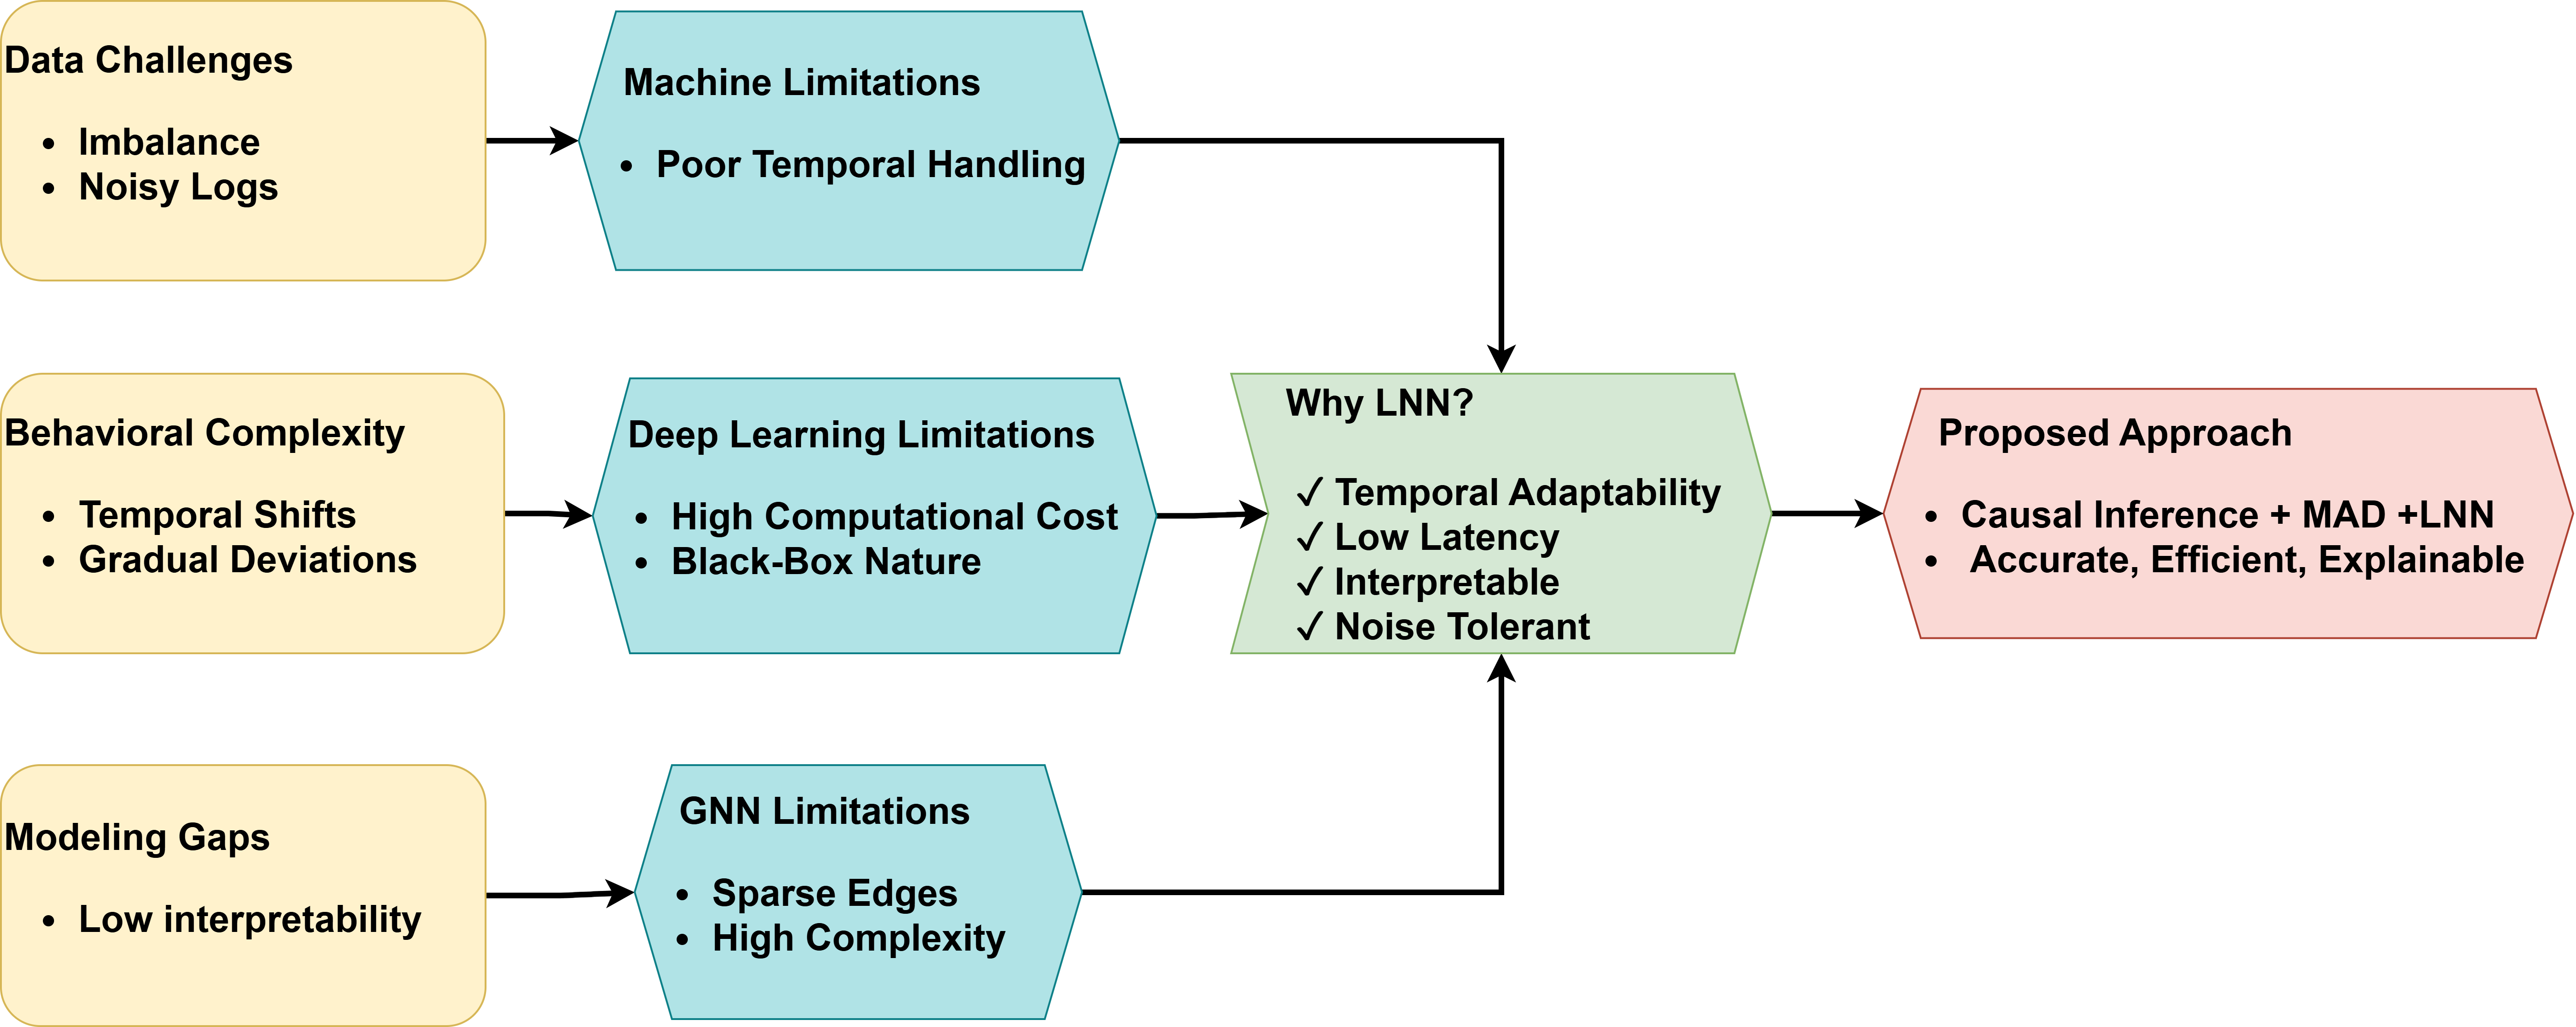
\includegraphics[width=1\linewidth]{figures/lnn_literature_survey_2_.png}
    \caption{Motivation for LNN}
    \label{lnn_suevey}
\end{figure}

The motivation and reasoning for embracing an LNN-based solution for insider threat detection problems shown in Figure \ref{lnn_suevey}. It starts with recognising major hindrances in three areas: data issues like imbalance and noisy logs, behavioral complexity with temporal changes and slow drifts, and modeling deficiencies characterised by low interpretability. These limitations result in constraints of conventional machine learning (poor time management), deep learning (expensive and black-box nature), and graph neural networks (sparse, high-level structures). To address this, LNN comes forth as a compelling alternative given its merits in temporal flexibility, low latency, interpretability, and robustness towards noise. The proposed method combines causal inference and MAD with LNN to provide a precise, efficient, and explainable detection system.


LNNs have emerged as a robust solution for noisy and time-varying settings with state-of-the-art performance in tasks ranging from time-series forecasting \cite{akpinar2025novel, hasani2021liquid}, signal classification \cite{cantini2025exact}, biomedical diagnosis and temporal knowledge inference \cite{han2025robust}, wireless communications \cite{wang2024robust}. Their ability to dynamically adapt to evolving inputs and framework continuous-time behaviors through differential equations makes them especially well-suited to approach the dynamic nature of insider threats. LNNs stand apart from traditional approaches in that they run at low computational cost, can process noisy or missing input streams, and preserve temporal memory, which is required for keeping track of real-time behavior. These features make them especially well-suited to insider threat detection, where subtle changes in behavior over time require accurate, adaptive responses.

The supervised learning strategy in this study, since pre-labeled user behavior between malicious and non-malicious is given in the CERTr4.2 dataset. This permits precise testing and training of classification approaches. Yet, conventional supervised approaches are temporally rigid and interpretable, both essential while insider threats unfolding over time and being driven by contextual and causal reasons. To overcome these issues, introduced a new approach, MAD based LNN, which combines LNNs' temporal reasoning powers with logical and causal interpretability. This framework permits strong, real-time insider threat detection even in noisy, imbalanced, or partially observable behavioral data settings.

\chapter{Theoretical Background and Requirements}\label{background}

\subsection{Causal Inference}
A causal method is a statistical framework \cite{zhao2023causal, naser2023causality} used to estimate causal effects from observational data by identifying and quantifying the relationship between variables and target. Here, the method is initialized with the provided dataset, which includes treatment variables (features) and an outcome variable (target label). In causal inference, the term "treatment" refers to the independent variables, or features, that are believed to influence the outcome. These variables are typically manipulated to understand the impact on the target label, and on the other hand, the dependent variable seeks to predict or explain. By analyzing this relationship, the causal method aims to estimate how changes in the treatment variables can lead to changes in the outcome, helping to uncover underlying causal relationships within the data.

In causal inference, the goal is to identify the causal effect of a treatment on an outcome. Eq. \ref{eq1} serves as the fundamental causal method, guiding the estimation of treatment effects in observational data settings.
\begin{equation}\label{eq1}
Y = f(X, U)
\end{equation}


$Y$ is the outcome variable (target label), $X$ represents the treatment (features), and $U$ represents any unobserved confounders or variables that might influence both $X$ and $Y$.

The causal relationship aims to estimate how a change in $X$ (the treatment) will cause a change in $Y$ (outcome). The challenge is to correctly identify and adjust for any confounding variables $U$, which may distort the true causal effect. 


\subsection{Linear Regression for Estimating the Causal Effect}

Linear regression is a common method used to estimate causal effects \cite{wang2015visual} in observational data by the relationship between an outcome variable (\(Y\)) and one or more predictor variables (\(X\)). The general form of the regression equation is, shown in Eq. \ref{eq2}.

\begin{equation}
Y = \beta_0 + \beta_1 X + \beta_2 U + \epsilon
\label{eq2}
\end{equation}

\( Y \) is the outcome variable (insider threat occurrence), \( X \) is the treatment variable (user activity patterns, system access logs), \( U \) represents confounding variables (user role, prior behavior), \( \beta_0 \) is the intercept, representing the baseline level of \( Y \) when all predictors are zero, \( \beta_1 \) is the causal effect of \( X \) on \( Y \), which we aim to estimate, \( \beta_2 \) accounts for the effect of the confounder \( U \) on , \( Y \) and \( \epsilon \) is the error term, representing unmeasured factors that influence \( Y \).

Causal effect estimation focuses on determining the direct impact of the treatment variable (\(X\)) on the outcome (\(Y\)). The coefficient \(\beta_1\) represents this causal effect, indicating how changes in \(X\) influence \(Y\). If \(\beta_1\) is significantly different from zero, it suggests a strong relationship where variations in \(X\) lead to measurable changes in \(Y\). For instance, if insider threats (\(Y\)) increase with specific user actions (\(X\)), and this effect remains significant after accounting for confounding factors, it infers a causal relationship between user actions and insider threats. 

However, confounding variables (\(U\)) can distort this relationship by influencing both \(X\) and \(Y\). If not accounted for, they can introduce bias and lead to spurious correlations. The coefficient \(\beta_2\) captures the effect of \(U\) on \(Y\), ensuring that the estimated effect of \(X\) on \(Y\) is not misinterpreted. For example, if job roles (\(U\)) impact both system access frequency (\(X\)) and the likelihood of insider threats (\(Y\)), failing to adjust for them \(U\) may lead to incorrect conclusions about the effect of access frequency on security risks. By including it \(U\) in the method, it can more accurately estimate the true causal impact of \(X\) on \(Y\), independent of external confounding influences.

Causal inference helps us find what events may be causing unusual behavior. For example, using linear regression, the sudden rise in email activity leading to risky actions like accessing sensitive files can be observed. This helps us focus on real triggers, not just patterns.

\subsection{LNN with Binary Classification and Entropy Loss}

LNNs are a variant of Recurrent Neural Networks(RNN) inspired by biological neurons that dynamically adapt their behavior based on input. Unlike traditional DL methods with fixed weights, LNNs employ time-dependent differential equations, making them highly effective for sequential and time-series tasks.

\subsubsection{LNN Dynamics}
The LNN dynamics of neural networks \cite{hasani2021liquid} have time-dependent differential equations that control how hidden states change over time. Traditional feedforward neural networks use fixed weights and change over time based on the input sequence. This tasks with sequential and time-series data, where the time-based changes are very important \cite{akpinar2025novel, han2025robust}.

The LNNs describe the network's state at a time \( t \) as a function of the previous state \( h(t-1) \), the current input \( x(t) \), and the network parameters \( w \). The hidden state at time \( t \), represented as \( h(t) \), changes based on a differential that models how components interact with each other over time, as shown in Eq. \ref{eq3}.


\begin{equation}\label{eq3}
\frac{d h(t)}{dt} = f(h(t), x(t), w)
\end{equation}
The hidden state at time \( t \) is \( h(t) \), the input is \( x(t) \), the learned parameters are \( w \), and \( f(\cdot) \) is a non-linear function that controls how the state changes. The method is flexible because it can change the weights based on changes in the input, which makes it more useful in real-world situations.

 LNNs are suited for this specific task because they can learn from instances as well as respect logical rules. With this facility, predetermined policies, for example, "no file sharing outside working hours," can be incorporated into the system. Thus, LNNs make the system more intelligent and explainable, which are essential in insider threat identification.

The sigmoid activation function is  used here, as it transforms real-valued outputs into a probability range between 0 and 1. This makes it ideal for problems where the output represents the likelihood of belonging to a particular class as represented in Eq. \ref{eq4}. The sigmoid function ensures that outputs are interpreted as probabilities, making it ideal for binary classification.

\begin{equation}\label{eq4}
\sigma(z) = \frac{1}{1 + e^{-z}}
\end{equation}

\( z \) is the weighted sum of inputs, which is shown in Eq. \ref{eq5}.
\begin{equation}\label{eq5}
z = W^T x + b
\end{equation}
\( W \) is the weight vector, \( x \) is the input feature vector and \( b \) is the bias term.


Binary Cross-Entropy (BCE) is used as loss function here for binary classification of insider and normal employee. It measures the dissimilarity between predicted probabilities and actual labels, guiding the method to improve its predictions, shown in Eq. \ref{eq6}.

\begin{equation}\label{eq6}
L = - \frac{1}{N} \sum_{i=1}^{N} \left[ y_i \log(\hat{y}_i) + (1 - y_i) \log(1 - \hat{y}_i) \right]
\end{equation}

Here \( N \) is the number of training samples, \( y_i \) is the actual label (0 or 1) and \( \hat{y}_i \) is the predicted probability obtained from the sigmoid function.

This loss function increases the penalty for wrong answers when the method is very confident. This helps the method learn to make more accurate and reliable predictions.

LNNs are superior than regular RNNs, GRUs, or LSTMs at finding insider threats because they use differential equations to model continuous-time dynamics. Due to their adaptive hidden states weighing strategy it easier to keep track of small changes in users behavior over time than methods that only look at one time step. This is very important for finding subtle, long-term insider activity that other methods might miss or make too simple.

\chapter{Proposed Methodology and System Design}\label{proposed}
A novel framework for insider threat detection that combines causal analysis + MAD-based feature refinement + SMOTE + LNNs is proposed which aims to effectively identify hidden behavioral patterns and respond to changes in user activity within an organization from user activity logs. 

\begin{figure}[!ht]
\centering
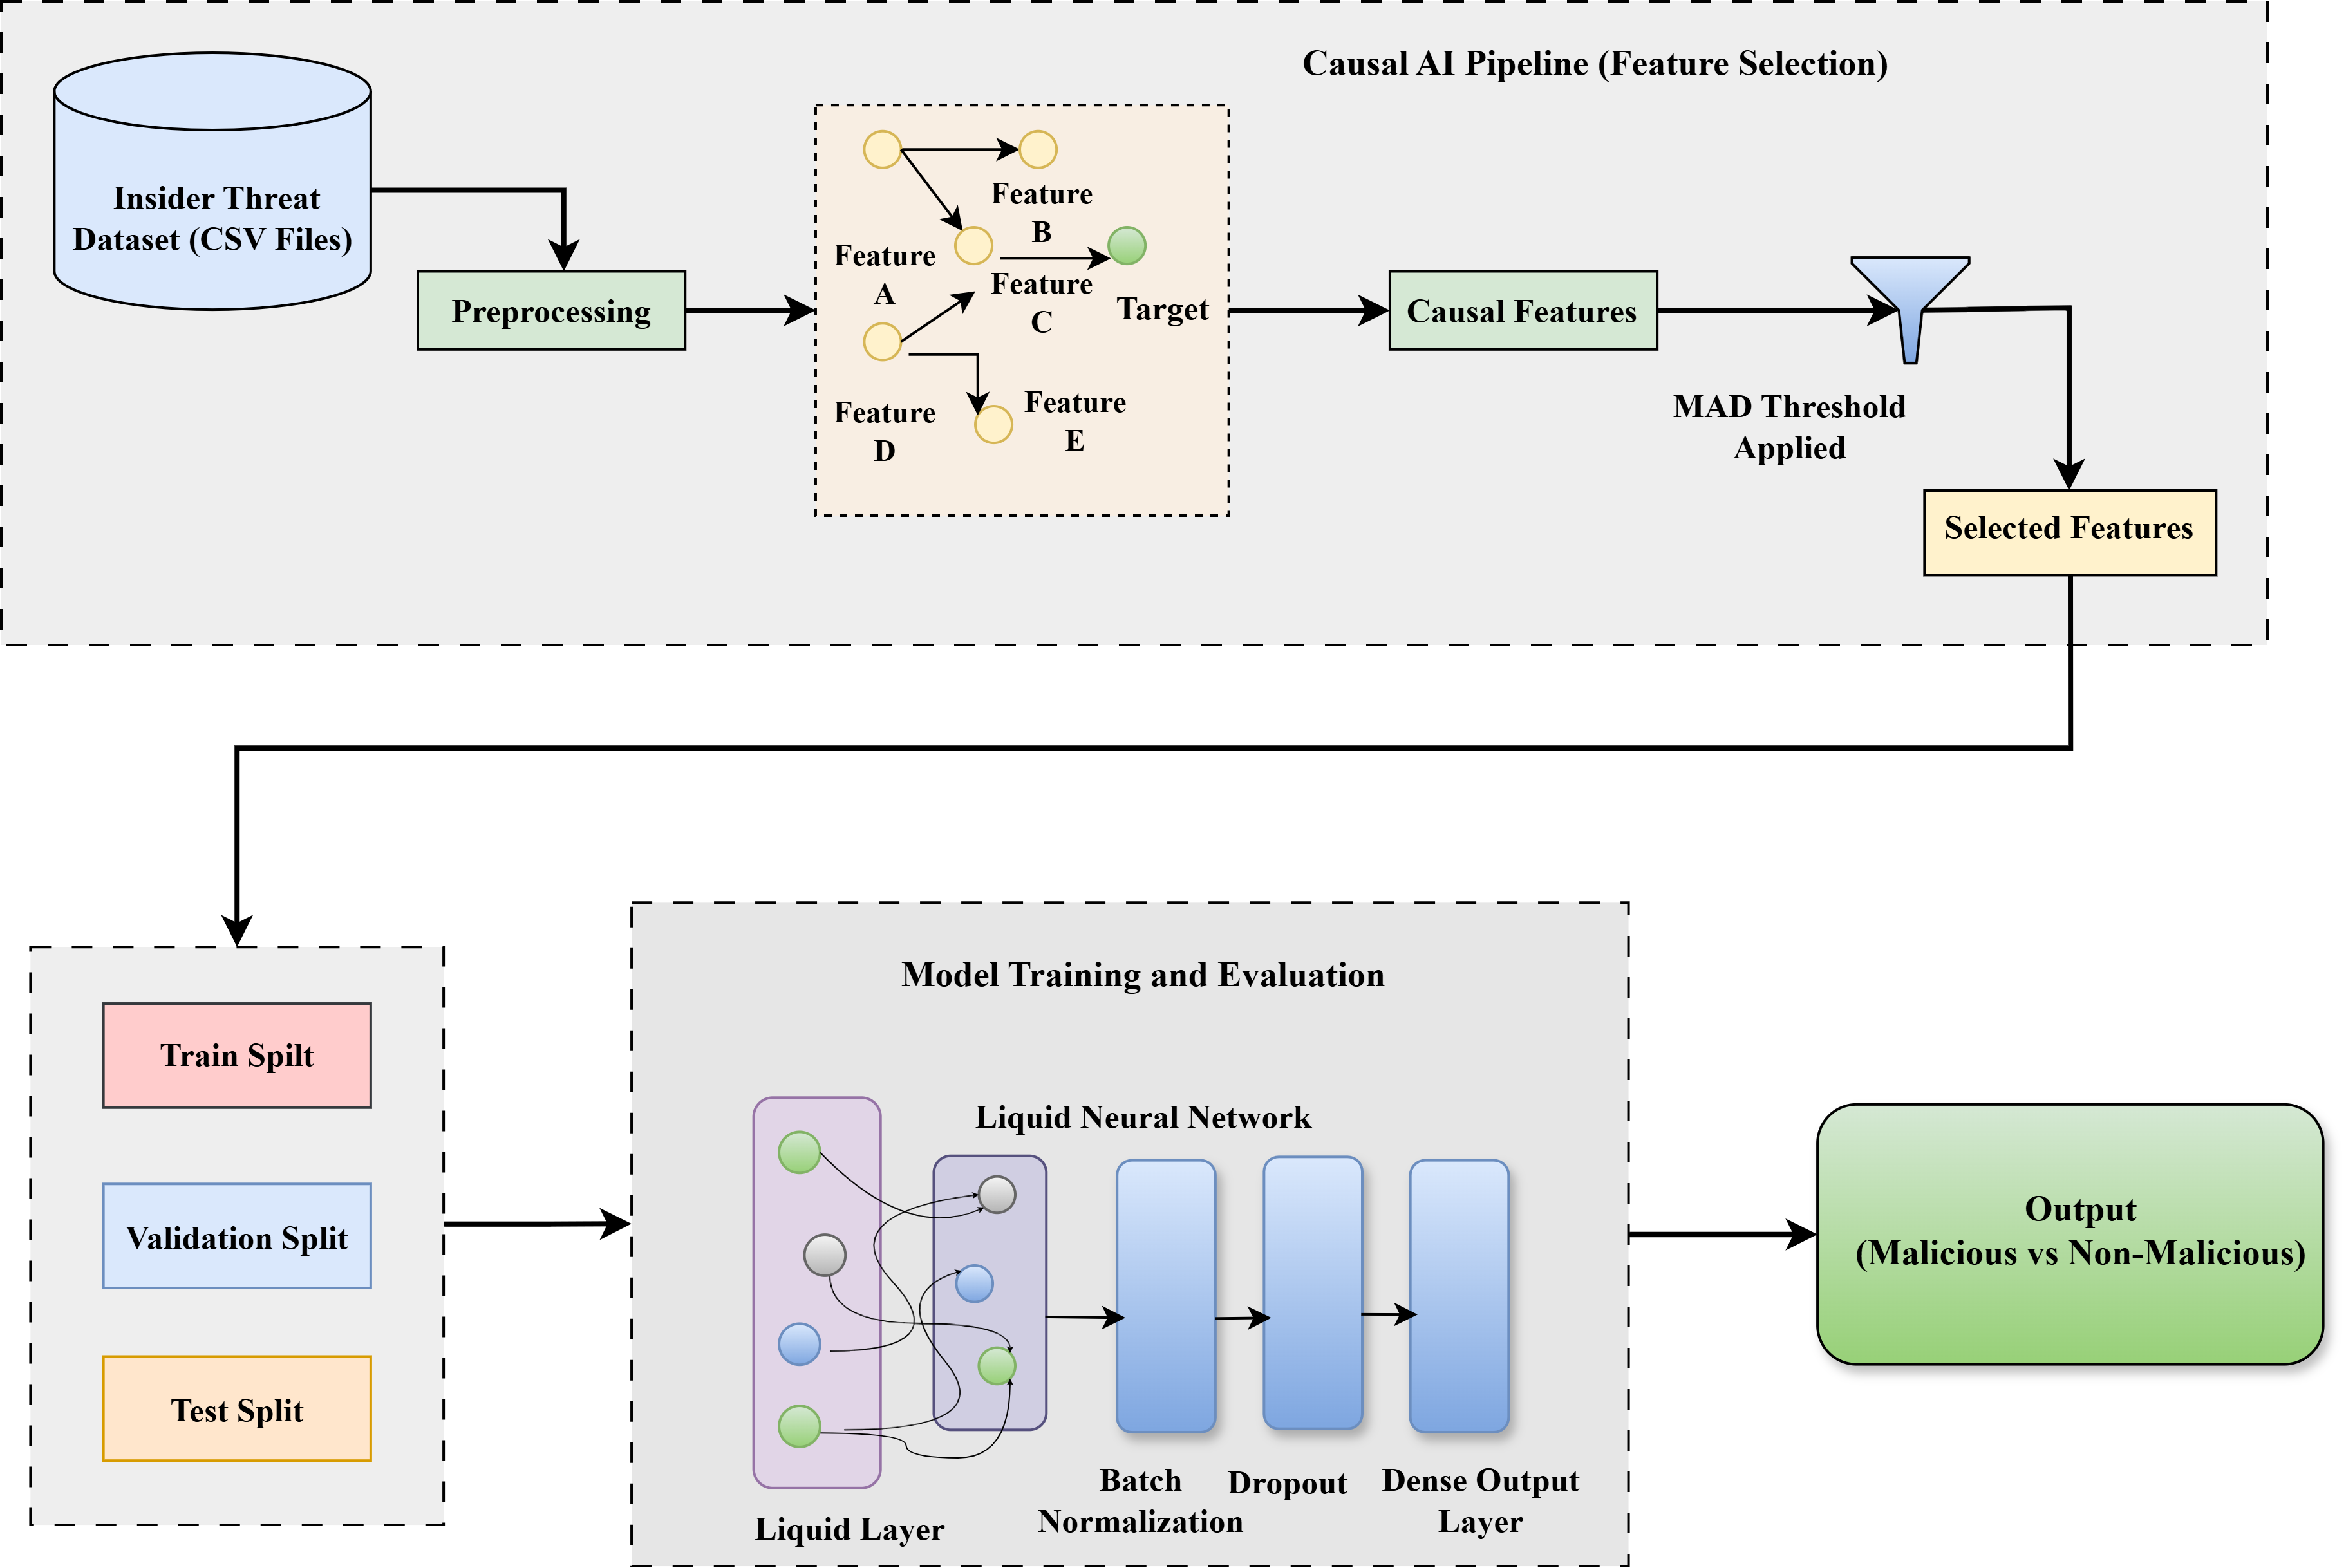
\includegraphics[width=0.95\textwidth,height=0.65\textwidth]{figures/Causal_LNN_1_.png}
\caption{Architecture of the Proposed Method}\label{fig1}
\end{figure}

Figure \ref{fig1} illustrates the proposed architecture, which begins with the collection of insider threat dataset files in  Comma Separated Values (CSV) format, which are then preprocessed. The preprocessed data is then subjected to feature selection through a Causal inference pipeline that performs relationships between features and the target variable. The causal features are filtered with a MAD threshold to select the most useful ones. These features are then divided into training, test, and validation sets. SMOTE is applied on train data for balancing both target classes. The central model is an LNN that handles the data with layers of batch normalization, dropout, and a dense output layer. Lastly, the model outputs whether the input was malicious or non-malicious behavior.





\subsection{Dataset}
The CERTr4.2 dataset is a well-known dataset from CMU for insider threat detection. It simulates real-world workplace activities, including both normal and malicious behavior. The dataset contains user activity logs such as file access, emails, logins, and website visits, which provide insights into employee behavior. It also has psychometric features that measure personality traits, state of mind, and behavioral habits. These features help us understand the psychological factors which can lead to insider behavior.  From both a technical and psychological point of view, each file gives us useful information about how users act. 
\begin{algorithm}
\caption{Insider Threat Detection via Causal Feature Selection and LNNs}\label{alg2}
\DontPrintSemicolon
\LinesNumbered
\small
\KwInput{CERT r4.2 Dataset $\mathcal{D}$ with $n$ samples and $m$ features}
\KwOutput{Classification metrics and confusion matrix}

\vspace{0.3cm}
\textbf{Step 1: Preprocessing (refer Algorithm~\ref{alg1})} \\
\Indp
Apply Session-wise, Day-wise, or Behavior-wise Preprocessing to $\mathcal{D}$\;
Obtain preprocessed feature matrix $X \in \mathbb{R}^{n \times m}$ and label vector $y \in \{0,1\}^n$\;
\Indm

\vspace{0.2cm}
\textbf{Def} \text{CausalFeatureSelection}$(X, y)$:\ \\
\Indp \ForEach{feature $f$ in $X$}{
    Estimate causal effect of $f$ on $y$ using DoWhy\;
}
Apply MAD threshold to select important features\;
\Indm \Return{$X_{sel} \in \mathbb{R}^{n \times m'}$}

\vspace{0.2cm}
\textbf{Def} \text{DataSplitBalanceStandardize}$(X_{sel}, y)$:\ \\
\Indp
Split $(X_{\text{sel}}, y)$ into train/val/test (70/15/15, stratified)\;
Apply SMOTE to training set\;
Reshape $X_{train}, X_{val}, X_{test}$ to $\mathbb{R}^{n \times T \times d}$ format\;
\Indm \Return{$X_{train}, y_{train}, X_{val}, y_{val}, X_{test}, y_{test}$}

\vspace{0.2cm}
\textbf{Def} \text{TrainLNN}$(X_{\text{train}},\ y_{\text{train}},\ X_{\text{val}},\ y_{\text{val}})$:\ \\
\Indp
for LNN Training (\textbf{refer to Algorithm \ref{algo2}) } \\
\Indm \Return{Trained method $f_{\text{LNN}}$}

\vspace{0.2cm}
\textbf{Def} \text{Evaluatemethod}$(f_{\text{LNN}}, X_{test}, y_{test})$:\ \\
\Indp Predict $\hat{y} \gets f_{\text{LNN}}(X_{test})$\;
Compute performance metrics \;
\Indm \Return{Evaluation report}

\vspace{0.2cm}
\textbf{Function} \text{Main()}:\ \\
\Indp $X, y \gets \text{LoadData}(\mathcal{D})$\;
$X_{sel} \gets \text{CausalFeatureSelection}(X, y)$\;
$X_{train}, y_{train}, X_{val}, y_{val}, X_{test}, y_{test} \gets \text{DataSplitBalanceStandardize}(X_{sel}, y)$\;
$f_{\text{LNN}} \gets \text{TrainLNN}(X_{train}, y_{train}, X_{val}, y_{val})$\;
$\text{metrics} \gets \text{Evaluatemethod}(f_{\text{LNN}}, X_{test}, y_{test})$\;
\Indm \Return{Final metrics and evaluation report}
\end{algorithm}
 The CERTr4.2 dataset is used, and data is preprocessed using three different methods: Session-wise, Day-wise, and Behavior-wise Preprocessing representations, which are explained in Algorithm \ref{alg2}.  These preprocessing methods find important patterns in temporal activity, which helps the method tell the difference between normal and bad behavior.
 
\begin{enumerate}

\item  logon.csv – keeps track of when users log in and out of the system.
\item device.csv – keeps track of how external storage devices, like USB drives, are used.
\item email.csv – keeps track of the emails that users send and receive.
\item file.csv – keeps track of how files are accessed and changed.
\item http.csv—has information about how users browse the web.
\item psychometric.csv – score of users' personalities and actions.
\item ldap.csv – keeps track of changes to user roles and the structure of the organization.
\end{enumerate}





\begin{table}[!ht]
\centering
\caption{Overview of CMU-CERTr4.2 dataset}\label{tab5}%
\begin{tabular}{@{}ll@{}}
\toprule
    \textbf{CMU-CERTr4.2 Dataset} & \textbf{Number of Records}  \\
\midrule
Data Collection Period	& 17 months\\
Total Number of Users	& 1,000 Users\\
User Distribution	& 930 Non-malicious, 70 Malicious\\
Logon.csv	& 58,45,859\\
Email.csv	& 26,29,979\\
File.csv	& 44,55,581\\
Device.csv	& 4,05,380\\
Http.csv	& 2,84,34,423\\
Psychometric.csv & 1000 \\
Total Event Count	& 3,27,70,222\\
\bottomrule
\end{tabular}
\end{table}

Table \ref{tab5} shows that the synthetic dataset has been collected over a period of 500 days. Around 1000 user log files have been recorded and of which 70 were insiders. It includes three scenarios of insider threats which are described as follows: \\
\textbf{Scenario 1:}  Suspicious activity: Unsual working patterns of employees are recorded after or before office hours.\\
\textbf{Scenario 2:}  Job-Hunting Data Theft: An employee looking for a new job uses a thumb drive more often to steal data before quitting.\\ \textbf{Scenario 3:} Unauthorized Access and Sabotage: A user installs a keylogger, steals passwords, gains access, and sends a mass email to cause panic.

 The CMU-CERTr4.2 dataset is a synthetic dataset that may not fully capture the complexity and variability of real-world organizational environments, even though it does a efficient job of simulating how insiders act.  So, while it is efficient for controlled testing and comparing different ways to find insider threats, you should be careful when trying to apply the results to real business situations.
 
\begin{algorithm}
\DontPrintSemicolon
\LinesNumbered
\small

\KwIn{Raw log dataset $D = \{(x_i, t_i, u_i)\}_{i=1}^N$ \\ 
\hspace{1.2em} $x_i$: activity features,\quad $t_i$: timestamp,\quad $u_i$: user ID}
\KwOut{Structured sequences $\mathcal{S} = \{S_j\}_{j=1}^M$}

\vspace{0.2cm}
\textbf{Step 1: Chronological Ordering} \\
Sort $D$ by user and timestamp:\quad $D \gets \texttt{sort}(D, [u_i, t_i])$

\vspace{0.2cm}
\textbf{Step 2: Temporal Feature Extraction} \\
\ForEach{$x_i \in D$}{
    Compute weekday:\quad $d_i = \texttt{weekday}(t_i) \in \{0,1,\dots,6\}$\;
    Compute hour:\quad $h_i = \texttt{hour}(t_i) \in \{0,1,\dots,23\}$\;
    Assign temporal class:
    \[
    \tau_i =
    \begin{cases}
    1 & \text{if } d_i < 5 \land 9 \leq h_i < 17 \quad \text{(Weekday Work)}\\
    2 & \text{if } d_i < 5 \land h_i \notin [9,17) \quad \text{(Weekday After)}\\
    3 & \text{if } d_i \geq 5 \land 9 \leq h_i < 17 \quad \text{(Weekend Work)}\\
    4 & \text{otherwise} \quad \text{(Weekend After)}
    \end{cases}
    \]
}

\vspace{0.2cm}
\textbf{Step 3: Weekly Segmentation} \\
Partition $D$ by week:\quad $D = \bigcup_w D^{(w)}$

\vspace{0.2cm}
\textbf{Step 4: Session Identification} \\
\ForEach{user $u$ in week $D^{(w)}$}{
    Collect user logs: $\mathcal{T}_u^{(w)} = \{ t_i \}_{u_i = u, x_i \in D^{(w)}}$\;
    Segment $\mathcal{T}_u^{(w)}$ by logon/logoff or inactivity gaps:\;
    $\mathcal{T}_u^{(w)} = \bigcup_{k=1}^{K_u^{(w)}} \mathcal{T}_{u,k}^{(w)}$
}

\vspace{0.2cm}
\textbf{Step 5: Behavioral Feature Encoding} \\
\ForEach{event $x_i$}{
    Extract behavior features $\phi(x_i)$ depending on action type:\;
    \quad email $\rightarrow$ \{type, size, attachments\}\;
    \quad file $\rightarrow$ \{path, size, access mode\}\;
    \quad http $\rightarrow$ \{URL depth, category\}
}

\vspace{0.2cm}
\textbf{Step 6: Construct Final Dataset} \\
Sequence:\quad 
$S_j = \{(x_t, \phi(x_t), \tau_t)\}_{t=1}^{T_j}$

\vspace{0.2cm}
\Return $\mathcal{S} = \{ S_j \}_{j=1}^{M}$
\caption{Preprocessing and Feature Extraction}\label{alg1}
\end{algorithm}


\subsection{Preprocessing and Feature Extraction}
Preprocessing is a significant component in finding insider threats because it changes raw user activity data into structured formats that can be easily approached and analyzed.  This method uses the CMU CERTr4.2 dataset.  Three different preprocessing methods are used to make classification more accurate and detailed. Each method is meant to capture user behavior at different levels of time granularity, as shown in Algorithm \ref{alg1}.
\begin{table}[!ht]
\centering
\caption{CERTr4.2 dataset preprocessing statistics}
\begin{tabular}{p{9cm} p{4cm}}
\cmidrule(lr){1-2}
\textbf{Preprocessed Details} & \textbf{No. of Instances} \\ \cmidrule(lr){1-2}

\multicolumn{2}{c}{\textbf{Session-wise Instances}}\\
\cmidrule(lr){1-2}
Preprocessed Instances & 4,70,611 \\
\cmidrule(lr){1-2}
Normal instances & 4,69,497\\ 
\cmidrule(lr){1-2}
Insider instances & 1,114\\ 
\cmidrule(lr){1-2}
Feature vector-based instances & 124\\ 
\cmidrule(lr){1-2}
Refined Feature Vector & 52\\ 
\cmidrule(lr){1-2}

\multicolumn{2}{c}{\textbf{Day-wise Instances}} \\
\cmidrule(lr){1-2}
Preprocessed Instances & 3,30,452 \\
\cmidrule(lr){1-2}
Normal instances & 3,29,486\\ 
\cmidrule(lr){1-2}
Insider instances & 966\\ 
\cmidrule(lr){1-2}
Feature vector-based instances & 504\\ 
\cmidrule(lr){1-2}
Refined Feature Vector & 205\\ 
\cmidrule(lr){1-2}
\multicolumn{2}{c}{\textbf{Behavioral Instances}}  \\
\cmidrule(lr){1-2}
Preprocessed Instances & 3,30,452 \\
\cmidrule(lr){1-2}
Normal instances & 3,29,486\\ 
\cmidrule(lr){1-2}
Insider instances & 966\\ 
\cmidrule(lr){1-2}
Feature vector-based instances & 25\\
\cmidrule(lr){1-2}
Refined Feature Vector & 13\\ 
\cmidrule(lr){1-2}

\end{tabular}
\label{tab4}
\end{table}
\begin{itemize}
    \item Session-wise Preprocessing splits user activity into different sessions that are based on interaction intervals which are continuous (active sessions). It is an accurate method that keeps short-term contextual behavior. It is most effective for locating suspicious behavior quickly in situations like a rapid file transfer or a strange command execution in an isolated activity window. Its detail level enables it to discover those threats that seem like short, tightly-concentrated user behavior bursts.

    \item In Day-wise Preprocessing, user activities are grouped into summaries that represent a compromise between detailed information and general trends. This way it is possible to detect local behavioral patterns that deviate from the usual, for example, logging in at unusual hours or accessing data more frequently on certain days. Essentially, the aim of the method is to illustrate daily behavioral changes which could, at very least, be an initial indication of bad behavior or breaches of the policy.

\item Behavioral-wise Preprocessing collects information about how users behave over longer periods of time, like a week for behavioral baselines. It is meant to find small changes in a user's normal behavior, like using more privileges over time or getting access to sensitive resources in a different way.  This is especially effective at catching insider attacks that move slowly and quietly and can get around short-term anomaly detectors.
\end{itemize}



To make it easier to understand, the causal feature extraction was added as an extra layer to each of the three preprocessing methods.  The causal inference method is used to find features that show cause-and-effect relationships with target class through statistical correlation.  This helps in selecting essential features for detecting insider with clearer and more justifiable decision-making. When used together with causal feature selection, these preprocessing methods make it possible to do multi-scale and causally informed behavioral analysis that can find both short-term and long-term anomalies.  This principled and layered method significantly improves the dependability and comprehensibility of insider threat detection systems.  Table \ref{tab4} shows the descriptive statistics for each of the three preprocessing methods.

\subsubsection{Causal Feature Selection}

The first step in the feature selection process is a causal analysis to find variables that have a direct effect on the target outcome.  This analysis measures how strong each feature's causal link to the dependent variable is by looking at both the direction (Cause–Effect) and the size (Absolute Effect).  Features that go above the MAD threshold are kept because they are causally significant.
\begin{table}[!ht]
\centering
\caption{Cause-effect sorted scores of selected features in Session-wise Preprocessing data}
\label{table4c}
\begin{tabular}{clc}
\toprule
\textbf{Sno} & \textbf{Feature} & \textbf{Score} \\
\midrule
1 & http\_n\_leakf & 0.99777920 \\
2 & http\_hackf\_mean\_url\_depth & 0.30074630 \\
3 & http\_leakf\_mean\_url\_depth & 0.24944480 \\
4 & http\_n\_hackf & 0.17561640 \\
5 & http\_hackf\_mean\_http\_c\_nwords & 0.02008966 \\
6 & http\_leakf\_mean\_http\_c\_nwords & 0.01936143 \\
7 & usb\_mean\_usb\_dur & 0.01284414 \\
8 & http\_hackf\_mean\_url\_len & 0.01216687 \\
9 & n\_days & 0.01208800 \\
10 & http\_leakf\_mean\_url\_len & 0.00915394 \\
11 & file\_phof\_n-disk1 & 0.00867041 \\
12 & file\_exef\_n-disk0 & 0.00776587 \\
13 & file\_n\_exef & 0.00715892 \\
14 & file\_txtf\_n-disk1 & 0.00413841 \\
15 & file\_docf\_n-disk2 & 0.00270463 \\
16 & http\_hackf\_mean\_http\_c\_len & 0.00248857 \\
17 & n\_usb & 0.00248043 \\
18 & isweekendafterhour & 0.00242713 \\
19 & file\_exef\_n-disk1 & 0.00236759 \\
20 & n\_logon & 0.00236741 \\
21 & start\_with & 0.00236741 \\ 22 & file\_exef\_n-disk2 & 0.00231611 \\ 23 & file\_compf\_n-disk2 & 0.00230449 \\ 24 & http\_leakf\_mean\_http\_c\_len & 0.00230030 \\ 25 & file\_txtf\_n-disk2 & 0.00224516 \\ 26 & file\_n-disk2 & 0.00222826 \\ 27 & file\_n-disk1 & 0.00221884 \\ 28 & file\_phof\_n-disk2 & 0.00216995 \\ 29 & file\_docf\_n-disk1 & 0.00214400 \\ 30 & file\_compf\_n-disk0 & 0.00213460 \\ (continues up to 52) &.....&.....\\ 52 & email\_mean\_n\_atts & 0.00023948 \\ \bottomrule
\end{tabular}
\vspace{0.2cm}
\scriptsize {\textbf{Note:} Total Features = 124, Selected = 52 (MAD Threshold = 0.000239)}
\end{table}

\begin{table}[!ht]
\centering
\caption{Cause-effect sorted scores of selected features in Day-wise Preprocessing data}
\label{table4d}
\begin{tabular}{clc}
\toprule
\textbf{Sno} & \textbf{Feature} & \textbf{Score} \\
\midrule
1 & workhourhttp\_leakf\_n-pc0 & 0.9970828 \\
2 & workhourhttp\_n\_leakf & 0.9970828 \\
3 & http\_leakf\_n-pc0 & 0.9691867 \\
4 & http\_n\_leakf & 0.9691867 \\
5 & afterhourhttp\_leakf\_n-pc0 & 0.9683666 \\
6 & afterhourhttp\_n\_leakf & 0.9683666 \\
7 & workhourlogon\_n-pc3 & 0.7970888 \\
8 & afterhourusb\_n-pc3 & 0.4971068 \\
9 & usb\_n-pc3 & 0.4971068 \\
10 & workhourallact\_n-pc3 & 0.4269069 \\
11 & logon\_n-pc3 & 0.3607731 \\
12 & afterhourlogon\_n-pc3 & 0.3171247 \\
13 & http\_hackf\_mean\_url\_depth & 0.3005814 \\
14 & workhourhttp\_hackf\_mean\_url\_depth & 0.3005814 \\
15 & http\_leakf\_mean\_url\_depth & 0.2493205 \\
16 & afterhourhttp\_leakf\_mean\_url\_depth & 0.2493190 \\ 17 & workhourhttp\_leakf\_mean\_url\_depth & 0.2492707 \\ 18 & http\_hackf\_n-pc0 & 0.1755198 \\ 19 & http\_n\_hackf & 0.1755198 \\ 20 & workhourhttp\_hackf\_n-pc0 & 0.1755198 \\ 21 & workhourhttp\_n\_hackf & 0.1755198 \\ 22 & allact\_n-pc3 & 0.1218024 \\ 23 & afterhourallact\_n-pc3 & 0.1137651 \\ 24 & workhourhttp\_leakf\_mean\_http\_c\_nwords & 0.02558419 \\ 25 & afterhourfile\_txtf\_n-disk1 & 0.02272044 \\ 26 & afterhourusb\_mean\_usb\_dur & 0.02066672 \\ 27 & http\_hackf\_mean\_http\_c\_nwords & 0.02007864 \\ 28 & workhourhttp\_hackf\_mean\_http\_c\_nwords & 0.02007864 \\ 29 & http\_leakf\_mean\_http\_c\_nwords & 0.01933054 \\ (continues up to 205) &.....&.....\\ 205 & afterhourfile\_mean\_file\_nwords & 0.00024333 \\ \bottomrule
\end{tabular}
\vspace{0.2cm}
\scriptsize{\textbf{Note:} Total Features = 504, Selected = 205 (MAD Threshold = 0.000241)}
\end{table}

\begin{table}[!ht]
\centering
\caption{Cause-effect sorted scores of selected features in Behavior-wise Preprocessing}
\label{table4b}
\begin{tabular}{clc}
\toprule
\textbf{Sno} & \textbf{Feature} & \textbf{Score} \\
\midrule
1 & H1\_norm & 1.007513 \\
2 & D1\_norm & 0.028600 \\
3 & D2\_norm & 0.024432 \\
4 & F1\_norm & 0.008956 \\
5 & L9\_norm & 0.007351 \\
6 & L6\_norm & 0.007169 \\
7 & L8\_norm & 0.007169 \\
8 & L4\_norm & 0.006423 \\
9 & L3\_norm & 0.006098 \\
10 & H3\_norm & 0.003707 \\
11 & H2\_norm & 0.003659 \\
12 & L7\_norm & 0.002980 \\
13 & C\_norm & 0.002848 \\
\bottomrule
\end{tabular}
\vspace{0.2cm}

\scriptsize{\textbf{Note:} Total Features = 25, Selected = 13 (MAD Threshold = 0.0028)}
\end{table}
To obtain more detailed behavioral dynamics across temporal contexts, the same causal MAD procedure is applied to Session-wise Preprocessing and Day-wise Preprocessing granularities within the CERT r4.2 dataset.  Table~\ref{table4c} shows the features that have a big impact on user behavior during a single work session, while Table~\ref{table4d} shows the bigger causal trends across daily activity patterns.  At the behavioral level, the causal–MAD filtering identifies the most significant behavioral indicators that facilitate insider threat detection, as outlined in Table~\ref{table4b}. 



By looking at the causal links between features and the target variable, only those that have a real causal effect are kept. This gets rid of any unnecessary or unrelated variables that could be used to predict insider threats.  After identifying the causal features, the MAD threshold is used to narrow down the choices even more.  MAD is a strong statistical method that looks at how different features vary. It is less affected by outliers than the standard deviation.  Using this two-stage causal-MAD filtering, the final features are both causally relevant and statistically significant. This makes the model easier to understand and more reliable for making predictions. After MAD refinement, the session based features are reduced from 124 to 52 which with MAD threshold value of 0.000239 as shown in Table~\ref{table4c}, day based features are refined from 504 to 205 with a MAD threshold value of 0.000241 as shown in Table~\ref{table4d} and behavioral features are refined from 25 to 13 with a MAD threshold value of 0.0028 as shown in Table~\ref{table4b}. shows that out of the 26 initial behavioral features, 13 were kept after the behavioral instance preprocessing pipeline used causal and MAD-based refinement.

\subsection{Data Imbalance handling}

Following feature selection, the dataset is divided into three subsets: 70\% for training, 15\% for validation, and 15\% for testing. This fixed split ensures that hyperparameters are tuned on the validation set, and final performance is reported on an unseen test set. To address class imbalance in the insider threat dataset, SMOTE is applied only on the training data to prevent data leakage. We chose this oversampling method over simple under-sampling because it keeps the information about the majority class and keeps important data from being lost. Also, the validation and test sets show the real distribution of the data so that the evaluation is fair.

\subsection{LNN Architecture Overview}
Figure~\ref{Fig2} shows the internal structure of LNN, which is designed to adapt to behavioral time-series data in order to find insider threats.  The network's input is a sequential data tensor with the shape \((128, 100, F)\). The batch size is 128, the number of temporal steps (or consecutive user activity windows) is 100, and the number of features F depends on the data type: 52 for Session-wise Preprocessing, 205 for Day-wise Preprocessing, or 13 for behavioral features.  During a single forward pass, only one modality is used.

\begin{figure}[!ht]
\centering
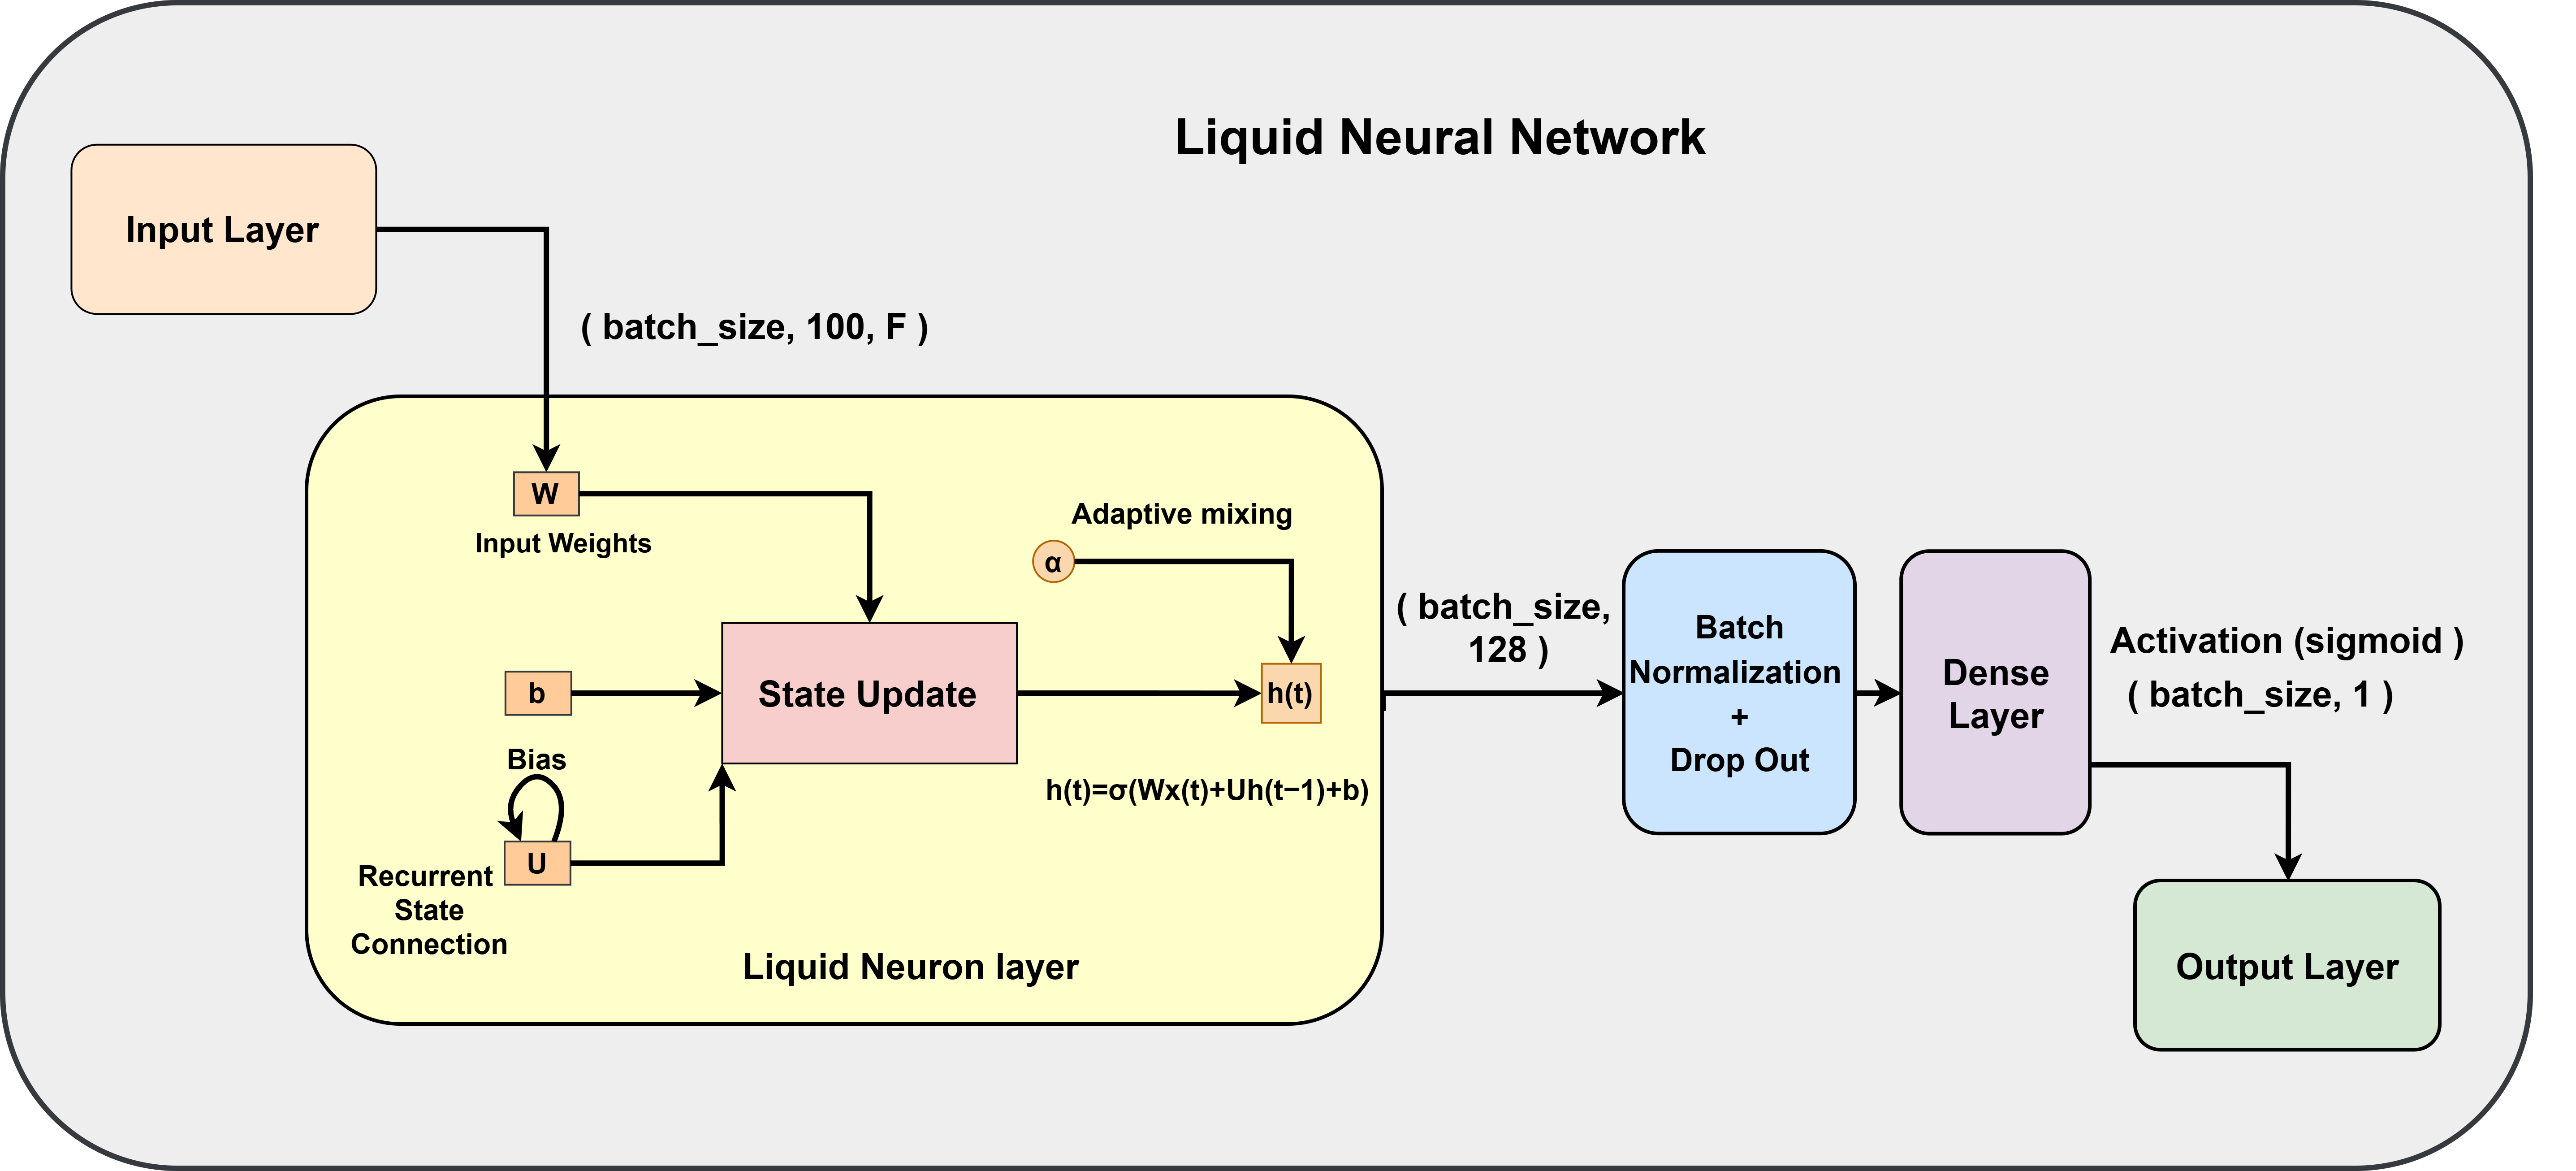
\includegraphics[width=1\textwidth,height=0.5\textwidth]{figures/lnn.png}
\caption{Internal Overview of LNN with Input/Output Dimensions and Activations }\label{Fig2}
\end{figure}


\begin{algorithm}[!ht]
\caption{LNN Model Training and Inference}
\label{algo2}
\DontPrintSemicolon
\KwIn{Input tensor $X \in \mathbb{R}^{128 \times 100 \times F}$, $F \in \{52, 205, 13\}$}
\KwOut{Binary predictions $Y \in \{0,1\}^{128}$}

\vspace{0.1cm}
\textbf{Def ForwardLNN}$(X)$: \tcp*{LNN forward computation}
\Indp
Initialize hidden state $h(0) \leftarrow \vec{0} \in \mathbb{R}^{128}$\;
\For{$t = 1$ \KwTo $100$}{
    Extract time slice $x(t) \in \mathbb{R}^{128 \times F}$ from $X$\;
    Compute hidden update:
    \[
    h(t) = \sigma(Wx(t) + Uh(t-1) + b)
    \]
    Apply adaptive mixing to refine $h(t)$\;
}
$H \leftarrow h(100) \in \mathbb{R}^{128 \times 128}$\;
Apply BatchNorm and Dropout to $H$\;
$Z = \text{Dense}(H) \in \mathbb{R}^{128 \times 1}$\;
$\hat{Y} = \sigma(Z)$ \tcp*{Sigmoid output}
\Indm
\Return{$\hat{Y}$}

\vspace{0.2cm}
\textbf{Def TrainLNN}$(X_{\text{train}}, y_{\text{train}}, X_{\text{val}}, y_{\text{val}})$:\ \\
\Indp
Initialize optimizer (Adam) and loss = \texttt{Weighted BCEWithLogitsLoss}\;
Train up to 100 epochs with batch size 128 and early stopping based on validation loss\;
Save best-performing checkpoint\;
\Indm
\Return{Trained model $f_{\text{LNN}}$}

\vspace{0.2cm}
\textbf{Def TestLNN}$(f_{\text{LNN}}, X_{\text{test}})$:\ \\
\Indp
$\hat{Y} \leftarrow f_{\text{LNN}}(X_{\text{test}})$\;
\For{$i = 1$ \KwTo $128$}{
    $Y_i \leftarrow (\hat{Y}_i \geq 0.5)$ \tcp*{1 = Malicious, 0 = Non-malicious}
}
\Indm
\Return{$Y$}
\end{algorithm}

The core computation is governed by the recurrent update rule:

\begin{equation}\label{eq7}
h(t) = \sigma(Wx(t) + Uh(t-1) + b)
\end{equation}


The input at time step \(t\) is represented by \(x(t) \in \mathbb{R}^F\), the input and recurrent weight matrices are represented by \(W \in \mathbb{R}^{F \times 128}\) and \(U \in \mathbb{R}^{128 \times 128}\), the bias term is represented by \(b \in \mathbb{R}^{128}\), and nonlinearity is introduced by \(\sigma = \tanh\).  To improve temporal adaptivity, a mixing mechanism which dynamically balances the impact of previous hidden states and new inputs, allowing the network to efficiently capture changing behavioral dynamics.






Each of the two stacked recurrent layers that make up the LNN architecture maintains a hidden state with dimensions of 128.  The final hidden representation \(h(100) \in \mathbb{R}^{128 \times 128}\) functions as a compact, temporally-aware embedding of user activity after processing all 100 time steps. This effectively summarizes long-term behavioral dependencies for insider threat classification as shown step by step in Algorithm~\ref{algo2}. Timely insider threat detection is made possible by the LNN's adaptive and recurrent nature, which enables the model to detect minute temporal variations in user behavior.

\chapter{Implementation and Experimental Setup} \label{setup}
The experiments were condcuted on HP Workstation with Windows operating system, powered by an Intel Core i7-10510U Central Processing Unit (CPU) running at 2.30 GHz, 32GB of RAM, and a 4GB Nvidia Quadro P520 Graphics Processing Unit (GPU), was used to conduct the insider threat detection experiments. Python libraries such as Dowhy for causal inference, TensorFlow for training LNNs, Scikit-learn for preprocessing and evaluation, NumPy and Pandas for data handling, and Matplotlib for plotting were used in the setup. Every experiment was carried out in the Anaconda environment using Jupyter Notebook.

The model was trained with a binary cross-entropy loss and a label smoothing factor of 0.03. 
AdamW was used for optimization with a learning rate of $1 \times 10^{-3}$, a weight decay of $1 \times 10^{-4}$, and a gradient clipping of 1.0, with Adam as a backup. 
To reduce residual skew, the balanced heuristic was used to compute class weights. 
Training was performed for up to 100 epochs with a batch size of 128 and a 15\% validation split. 
Early stopping monitored the validation loss for seven epochs and restored the best weights, while a ReduceLROnPlateau scheduler adjusted the learning rate (factor 0.5, patience 3, minimum $1 \times 10^{-6}$) to ensure stable convergence.

\subsection{Performance Metrics}
To evaluate the proposed method, the classification metrics comprises of Accuracy (Acc.), Precision (Pr.), Recall (Rec.), F1-score (F1.), ROC-AUC (AUC), FPR are considered. These metrics are calculated through the given from Eq. \eqref{eq29} to \eqref{eq33} with the help of the confusion matrix shown below in Figure \ref{Fig6}. where TP = True Positives, FP = False Positives, FN = False Negatives, and TN = True Negatives \cite{alslaiman2023enhancing}.

\begin{figure}[!ht]
\centering
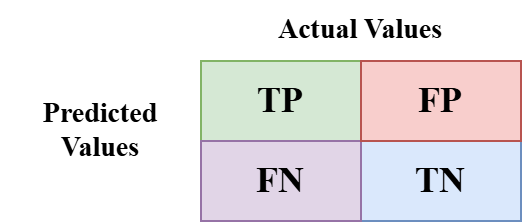
\includegraphics[width=0.6\textwidth,height=0.2\textwidth]{figures/figure6.png}
\caption{Confusion Matrix}\label{Fig6}
\end{figure}

\text{
Acc
}: The proportion of instances correctly classified out of the total.
\begin{equation}\label{eq29}
\text{Acc.} = \frac{\text{TP+TN}}{\text{TP+TN+FP+FN}}
\end{equation}

\text{Pr.}: The ratio of correctly predicted positives to the total predicted positives.
\begin{equation}\label{eq30}
\text{Pr.} = \frac{TP}{TP + FP}
\end{equation}

\text{Rec.}: The ratio of correctly identified positives to the total actual positives.
\begin{equation}\label{eq31}
\text{Rec.} = \frac{TP}{TP + FN}
\end{equation}

\text{F1-Score}: The balanced average of Precision and Recall, measuring a method's overall performance.
\begin{equation}\label{eq32}
\text{F1.} = 2 \times \frac{\text{Pr.} \times \text{Recall}}{\text{Pr.} + \text{Rec.}}
\end{equation}

\text Receiver Operating Characteristic Area Under the Curve: Represents the ability of the method to distinguish between positive and negative classes. 

\text{FPR}: The proportion of normal (negative) instances incorrectly classified as malicious (positive), indicating the false alarm rate.
\begin{equation}\label{eq33}
\text{FPR} = \frac{\text{FP}}{\text{FP} + \text{TN}}
\end{equation}

\chapter{Results and Discussion}\label{results}

\subsection{Training Convergence of the Proposed Method}
The training performance of a model we proposed under three different preprocessing granularity levels: session, day, and behavioral inputs. They looked at the convergence patterns by means of accuracy and loss curves to judge the stability and generalization of the model using 100 epochs with early stopping.
\begin{figure}[!ht]
\centering
\begin{minipage}[b]{0.48\textwidth}
\centering
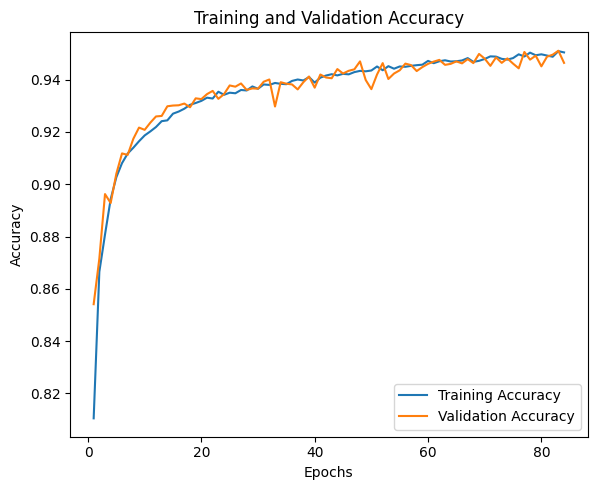
\includegraphics[width=\textwidth,height=0.7\textwidth]{figures/Session_LNN_Training_Accuracy_plot.png}
\end{minipage}
\hfill
\begin{minipage}[b]{0.48\textwidth}
\centering
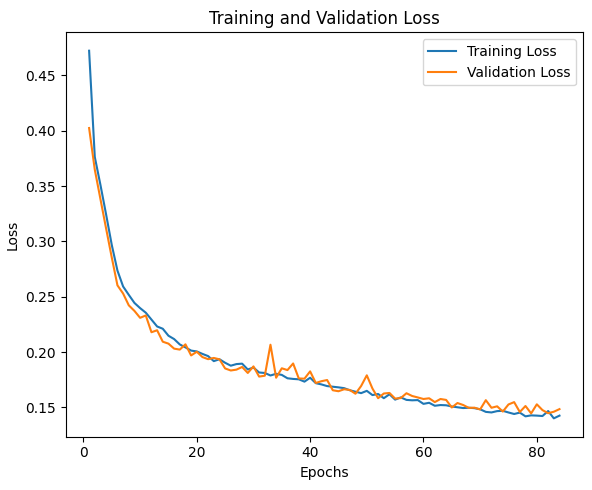
\includegraphics[width=\textwidth,height=0.7\textwidth]{figures/Session_LNN_Training_Loss_plot.png}
\end{minipage}
\caption{Training and validation accuracy (left) and loss (right) on Session-wise data.}
\label{fig:session_curves}
\end{figure}
Session-wise Preprocessing as shown in figure \ref{fig:session_curves} exemplifies the most rapid and stable convergence of the training. Within the first few epochs, the training accuracy goes up very fast, reaching a level above 95\% and stabilizing there, whilst the loss recedes rapidly and after that remains at a somewhat low level. So, session information seems to be the most effective way to capture temporal dependencies at the micro level, thus the network can identify very subtle behavioral anomalies with only a few training iterations.


\begin{figure}[!ht]
\centering
\begin{minipage}[b]{0.48\textwidth}
\centering
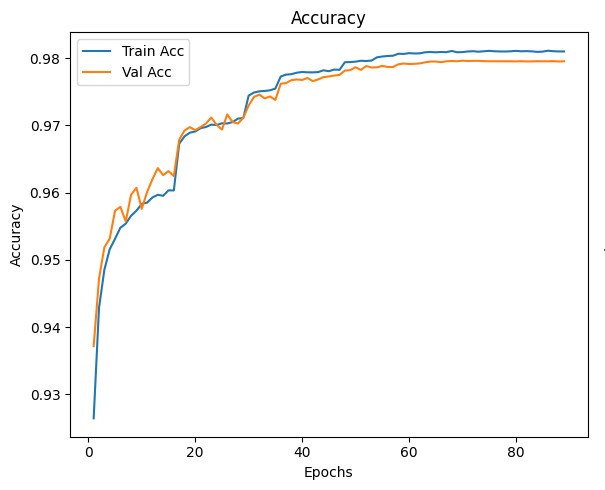
\includegraphics[width=\textwidth,height=0.7\textwidth]{figures/Day_LNN_Training_Accuracy_plot.png}
\end{minipage}
\hfill
\begin{minipage}[b]{0.48\textwidth}
\centering
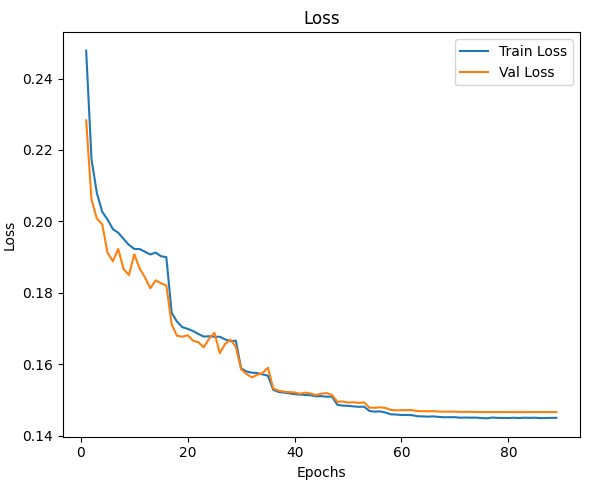
\includegraphics[width=\textwidth,height=0.7\textwidth]{figures/Day_LNN_Training_Loss_plot.png}
\end{minipage}
\caption{Training and validation accuracy (left) and loss (right) on Day-wise data.}
\label{fig:day_curves}
\end{figure}
Day-wise Preprocessing in figure \ref{fig:day_curves} tells a much more gradual convergence pattern. The accuracy gets superior in a steady manner and the loss drops quite slowly before it finally levels off. It can be seen that Day-wise Preprocessing inputs are of a broader temporal resolution and thus the model has to learn generalized daily activity trends. Although the convergence is slower, the final accuracy together with the low loss are the proof that Day-wise Preprocessing is able to capture the aggregated patterns of insider behavior.


\begin{figure}[!ht]
\centering
\begin{minipage}[b]{0.48\textwidth}
\centering
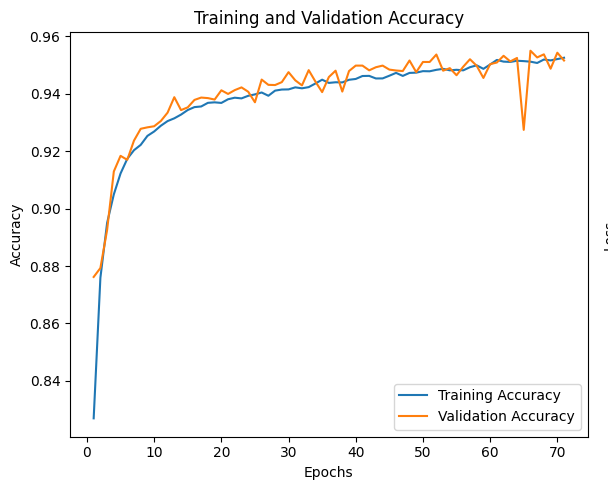
\includegraphics[width=\textwidth,height=0.7\textwidth]{figures/Behavior_LNN_Training_Accuracy_plot.png}
\end{minipage}
\hfill
\begin{minipage}[b]{0.48\textwidth}
\centering
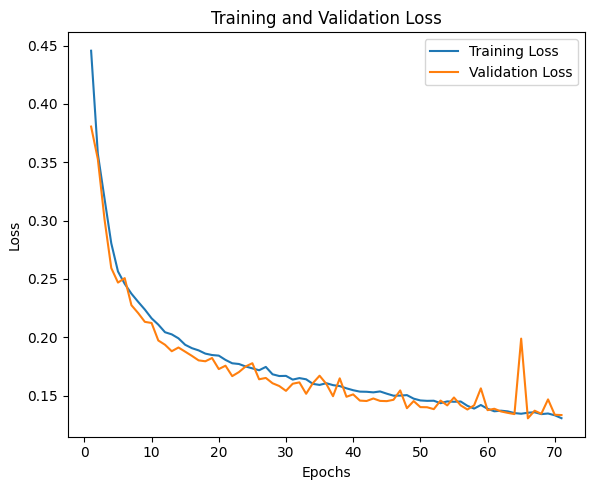
\includegraphics[width=\textwidth,height=0.7\textwidth]{figures/Behavior_LNN_Training_Loss_plot.png}
\end{minipage}
\caption{Training and validation accuracy (left) and loss (right) on Behavioral data.}
\label{fig:behavior_curves}
\end{figure}

Behavioral-wise Preprocessing in figure \ref{fig:behavior_curves} illustrates the slowest convergence. Here accuracy keeps getting gradually and finally it stabilizes at a resorting to a slightly lower level than the other two granularities. Those findings imply that long-term behavioral aggregation is a effective idea if one wants to find broader deviations but, at the same time, it may hide short-term variations and a longer training period is necessary so that the discriminator can recognize the patterns effectively.



Session-wise Preprocessing is capable of yielding the fastest and most precise convergence, thereby making it the most appropriate method for the detection of sudden insider anomalies requiring a very short training time. Preprocessing at the Day-wise Preprocessing is a compromise between interpretability and accuracy, whereas the Behavioral-wise Preprocessing, which is slower and less discriminative, is still useful for capturing ket-term changes in user behavior. 

\subsection{Scalability under Varying Data Ratios}
To investigate scalability, the proposed method was evaluated on 10\%, 15\%, 25\%, 50\%, 75\%, and 100\% data splits across session, day and behavior inputs. The results are divided into two tables for clarity: Table~\ref{tab:ratio_metrics} and Table~\ref{tab:ratio_stats} summarizes runtime efficiency and statistical validation.

\begin{table}[!ht]
\centering
\caption{Metrics evaluation of the proposed method across data ratios}
\label{tab:ratio_metrics}
\renewcommand{\arraystretch}{1.3}
\small
\begin{tabular}{|l|l|l|l|l|l|l|l|}
\hline
\textbf{Input} & \textbf{Data Ratio} & \textbf{Acc.} & \textbf{Prec.} & \textbf{Rec.} & \textbf{F1} & \textbf{AUC} & \textbf{FPR}\\
\hline
\multirow{6}{*}{Session} 
 & 10\%  & 95.79 & 96.08 & 95.47 & 95.78 & 99  & 3.90\\
\cline{2-8}
 & 15\%  & 95.96 & 95.32 & 96.67 & 95.99 & 99 & 4.75\\
\cline{2-8}
 & 25\%  & 96.25 & 96.11 & 96.39 & 96.25 & 99  & 3.90\\
\cline{2-8}
 & 50\%  & 96.60 & 95.57 & 97.73 & 96.64 & 99  & 4.53\\
\cline{2-8}
 & 75\%  & 97.23 & 96.80 & 97.70 & 97.24 & 99  & 4.17\\
\cline{2-8}
 & \textbf{100\%} & \textbf{97.98} & \textbf{97.30} & \textbf{98.71} & \textbf{98.00} & \textbf{99.6}  & \textbf{2.74}\\
\hline
\multirow{6}{*}{Day} 
 & 10\%  & 81.86 & 82.09 & 81.51 & 81.80 & 90  & 17.79\\
\cline{2-8}
 & 15\%  & 86.51 & 84.34 & 89.66 & 86.92 & 94  & 16.64\\
\cline{2-8}
 & 25\%  & 87.27 & 87.61 & 86.82 & 87.21 & 93  & 12.28\\
\cline{2-8}
 & 50\%  & 90.93 & 91.74 & 89.96 & 90.84 & 96  & 8.09\\
\cline{2-8}
 & 75\%  & 92.34 & 93.06 & 91.50 & 92.27 & 96  & 6.83\\
\cline{2-8}
 & \textbf{100\%} & \textbf{95.40} & \textbf{94.86} & \textbf{96.00} & \textbf{95.43} & \textbf{98}  & \textbf{5.20}\\
\hline
\multirow{6}{*}{Behavior} 
 & 10\%  & 94.60 & 94.68 & 94.52 & 94.60 & 98  & 5.31\\
\cline{2-8}
 & 15\%  & 94.97 & 94.45 & 95.55 & 95.00 & 99 & 6.13\\
\cline{2-8}
 & 25\%  & 95.12 & 94.02 & 96.38 & 95.18 & 99  & 5.61\\
\cline{2-8}
 & 50\%  & 95.93 & 95.04 & 96.91 & 95.97 & 99  & 5.05\\
\cline{2-8}
 & 75\%  & 96.27 & 95.38 & 97.25 & 96.30 & 99  & 4.71\\
\cline{2-8}
 & \textbf{100\%} & \textbf{96.57} & \textbf{96.36} & \textbf{96.80} & \textbf{96.58} & \textbf{99}  & \textbf{3.66}\\
\hline
\end{tabular}

\vspace{2mm}
\scriptsize{\textit{Note: Bold rows indicate the highest performance under each preprocessing input.}}
\end{table}


The performance improves consistently with increasing data ratio across all input granularities. At the Session-wise Preprocessing, performance is already near-saturated at low data ratios: accuracy moves only from 95.79\% (10\%) to 97.98\% (100\%), FPR reduces from 3.90 (10\%) to 2.74 (100\%), and ROC–AUC remains almost flat at $\sim$99. This shows that even with limited data availability, Session-wise Preprocessing representations are able to capture highly discriminative user behavior. Accuracy for Day-wise Preprocessing inputs rises from 81.86\% at 10\% of the data to 95.40\% at full data, with the F1-score improving concurrently (81.80 to 95.43) and FPR decreasing from 17.79 to 5.20 at 100\%. These results show that having more data makes it easier to find user-level temporal variations. The ROC–AUC keeps fluctuating between 98 and 99, and the behavior-wise Preprocessing performance is also stable, improving from 94.60\% to 96.57\% across data ratios, with FPR consistently declining from 5.31 to 3.66.

\begin{table}[!ht]
\centering
\caption{Statistical validation of LNN-CMSM across data ratios}
\label{tab:ratio_stats}
\renewcommand{\arraystretch}{1.3}
\small
\begin{tabular}{|l|l|l|l|l|}
\hline
\textbf{Input} & \textbf{Data Ratio} & \textbf{Training Time (s)} & \textbf{T-test} & \textbf{F-test} \\
\hline
\multirow{6}{*}{Session} 
 & 10\%  & 73.35 & 1109.49 & 1230959.63 \\
\cline{2-5}
 & 15\%  & 113.10 & 1156.66 & 1337858.63 \\
\cline{2-5}
 & 25\%  & 122.19 & 1190.75 & 1417898.38 \\
\cline{2-5}
 & 50\%  & 133.40 & 1267.78 & 1607259.75 \\
\cline{2-5}
 & 75\%  & 159.40 & 1410.88 & 1990587.00 \\
\cline{2-5}
 & \textbf{100\%} & \textbf{470.07} & \textbf{1651.99} & \textbf{2729064.25} \\
\hline
\multirow{6}{*}{Day} 
 & 10\%  & 27.07 & 359.33 & 129114.54 \\
\cline{2-5}
 & 15\%  & 42.98 & 457.11 & 208952.66 \\
\cline{2-5}
 & 25\%  & 67.75 & 451.01 & 203412.14 \\
\cline{2-5}
 & 50\%  & 147.74 & 564.35 & 318490.38 \\
\cline{2-5}
 & 75\%  & 162.51 & 620.84 & 385438.16 \\
\cline{2-5}
 & \textbf{100\%} & \textbf{214.07} & \textbf{856.73} & \textbf{733988.06} \\
\hline
\multirow{6}{*}{Behavior} 
 & 10\%  & 73.88 & 810.95 & 657640.13 \\
\cline{2-5}
 & 15\%  & 80.20 & 837.58 & 701535.81 \\
\cline{2-5}
 & 25\%  & 88.46 & 859.55 & 738824.69 \\
\cline{2-5}
 & 50\%  & 156.11 & 945.10 & 893213.06 \\
\cline{2-5}
 & 75\%  & 250.64 & 1006.18 & 1012392.75 \\
\cline{2-5}
 & \textbf{100\%} & \textbf{349.44} & \textbf{1069.14} & \textbf{1143054.88} \\
\hline
\end{tabular}

\vspace{2mm}
\scriptsize{\textit{Note: Bold rows correspond to the peak efficiency and statistical separation.}}
\end{table}

Table~\ref{tab:ratio_stats} adds to these results by showing the time spent training and the results of the statistical tests. As expected, runtime goes up as the size of the data goes up, but the increases are still small compared to the gains in accuracy and F1. For instance, the time it takes to train a session goes from 73.35 seconds (10\%) to 470.07 seconds (100\%). This increase is reasonable because it clearly improves performance. The T-test values get higher as the data ratio goes up, which means that the statistical difference between reduced and full data conditions gets stronger. The F-test values are also consistently large, around $10^{5}$–$10^{6}$, which shows that the performance improvements we saw are not random but systematic. The highest values are obtained at full data, especially for the session input (T-test = 1651.99; F-test = 2729064.25), which shows that the integrated method is strong. These results show that the proposed method works well with more data and stays strong when there isn't much data. Session-wise Preprocessing inputs provide the most consistent and distinct performance, closely followed by Behavior-wise Preprocessing inputs, while Day-wise Preprocessing inputs gain the most from larger data sets.

\begin{table}[!ht]
\centering
\caption{ANOVA summary statistics across preprocessing variants.}
\label{tab:anova_summary}
\renewcommand{\arraystretch}{1.3}
\small
\begin{tabular}{|l|l|l|l|l|}
\hline
\textbf{Metric} & \textbf{F(2,27)} & \textbf{p-value} & \textbf{$\eta^2$} & \textbf{Significant Pairs (Tukey HSD)} \\ \hline
Accuracy & 18.42 & $<$0.001 & 0.81 & Session–Day, Session–Behavior ($p<0.01$) \\ \hline
Precision & 15.76 & $<$0.001 & 0.78 & Session–Day, Session–Behavior ($p<0.01$) \\ \hline
Recall & 1.92 & 0.164 & 0.12 & None \\ \hline
F1-Score & 17.33 & $<$0.001 & 0.80 & Session–Day, Session–Behavior ($p<0.01$) \\ \hline
AUC & 21.05 & $<$0.001 & 0.84 & Session–Day ($p<0.01$), Session–Behavior ($p<0.05$) \\ \hline
\end{tabular}

\vspace{1mm}
\scriptsize{\textit{Note: $\eta^2$ denotes effect size. Significant pairs identified using Tukey’s HSD post-hoc test ($\alpha = 0.05$).}}
\end{table}


Table~\ref{tab:anova_summary} provides a detailed summary of the one-way ANOVA and post-hoc analysis results. The ANOVA confirms that the preprocessing type (\textit{i.e.}, Session, Day, or Behavior) has a statistically significant effect on all evaluation metrics (\textit{p} < 0.001), except Recall (\textit{p} > 0.05). The effect sizes ($\eta^2$) range from 0.78 to 0.84, which indicates a strong influence of preprocessing granularity on model performance. 

Post-hoc Tukey HSD tests further reveal that the Session-wise Preprocessing variant significantly outperforms both Day and Behavior-wise Preprocessing variants for Accuracy, Precision, F1-score, and AUC, with $p<0.01$. However, differences between Day and Be inputs are statistically insignificant, suggesting that both perform comparably when sufficient data are available. 

Together, these statistical results affirm that the Session-wise Preprocessing preprocessing contributes the most to overall performance improvements and that the proposed framework’s gains are consistent, statistically significant, and generalizable across input granularities.


\subsection{Cross-Dataset and Distinct User Evaluation}

In order to demonstrate the proposed method generalization more clearly, cross-dataset evaluations were carried out on benchmark CERT datasets (r5.2, and r6.2) under preprocessing inputs like session, day, and behavior data. The findings are given in Table~\ref{table11}. 

The model performed its best on the CERT r4.2, very notably under the Session-wise Preprocessing experiment (97.98\% accuracy and 99.6 AUC). The main point stressed in the Session-wise Preprocessing temporal sequences is that they contain the most behavioral changes and thus they are the best for insider threat recognition. 
And at the Day level tests the model's stability to even a greater extent whereby the accuracy moves from 95.40\% (r4.2) to 87.85\% (r6.2). Features at the Day-wise Preprocessing they still succeeded in differentiating datasets. 

Additionally, the model at r4.2 was also able to achieve efficient results (96.57\% accuracy, 99 AUC) at the Behavior-wise Preprocessing. Although there was a slight drop in the performance of the model on the new datasets (r5.2 and r6.2), the accuracies were still over 89\% and the AUC values were still over 90. This indicates that the system has become user behavior and dataset aware. 

\begin{table}[!ht]
\centering
\caption{Cross-dataset metrics evaluation of the proposed method.}
\label{table11}
\renewcommand{\arraystretch}{1.3} % slight row height
\setlength{\tabcolsep}{5pt}      % tighter columns
\small
\begin{tabular}{|l|l|l|l|l|l|l|}
\hline
\textbf{Input} & \textbf{Dataset} & \textbf{Acc.} & \textbf{Prec.} & \textbf{Rec.} & \textbf{F1} & \textbf{AUC} \\
\hline
\multirow{3}{*}{Session} 
 & r4.2 & \textbf{97.98} & \textbf{97.30} & \textbf{98.71} & \textbf{98.00} & \textbf{99.6} \\
\cline{2-7}
 & r5.2 & 92.80 & 93.10 & 92.30 & 92.70 & 94 \\
\cline{2-7}
 & r6.2 & 91.30 & 92.20 & 90.10 & 91.10 & 92 \\
\hline
\multirow{3}{*}{Day} 
 & r4.2 & \textbf{95.40} & \textbf{94.86} & \textbf{96.00} & \textbf{95.43} & \textbf{98} \\
\cline{2-7}
 & r5.2 & 91.20 & 89.80 & 92.50 & 91.10 & 93 \\
\cline{2-7}
 & r6.2 & 87.85 & 89.00 & 87.20 & 88.10 & 88 \\
\hline
\multirow{3}{*}{Behavior} 
 & r4.2 & \textbf{96.57} & \textbf{96.36} & \textbf{96.80} & \textbf{96.58} & \textbf{99} \\
\cline{2-7}
 & r5.2 & 90.50 & 91.20 & 89.30 & 90.20 & 91 \\
\cline{2-7}
 & r6.2 & 89.40 & 88.20 & 90.50 & 89.30 & 90 \\
\hline
\end{tabular}

\vspace{2mm}
\scriptsize{\textit{Note: Bold values indicate the best performance for each input across datasets.}}
\end{table}

\begin{figure}[!ht]
    \centering
    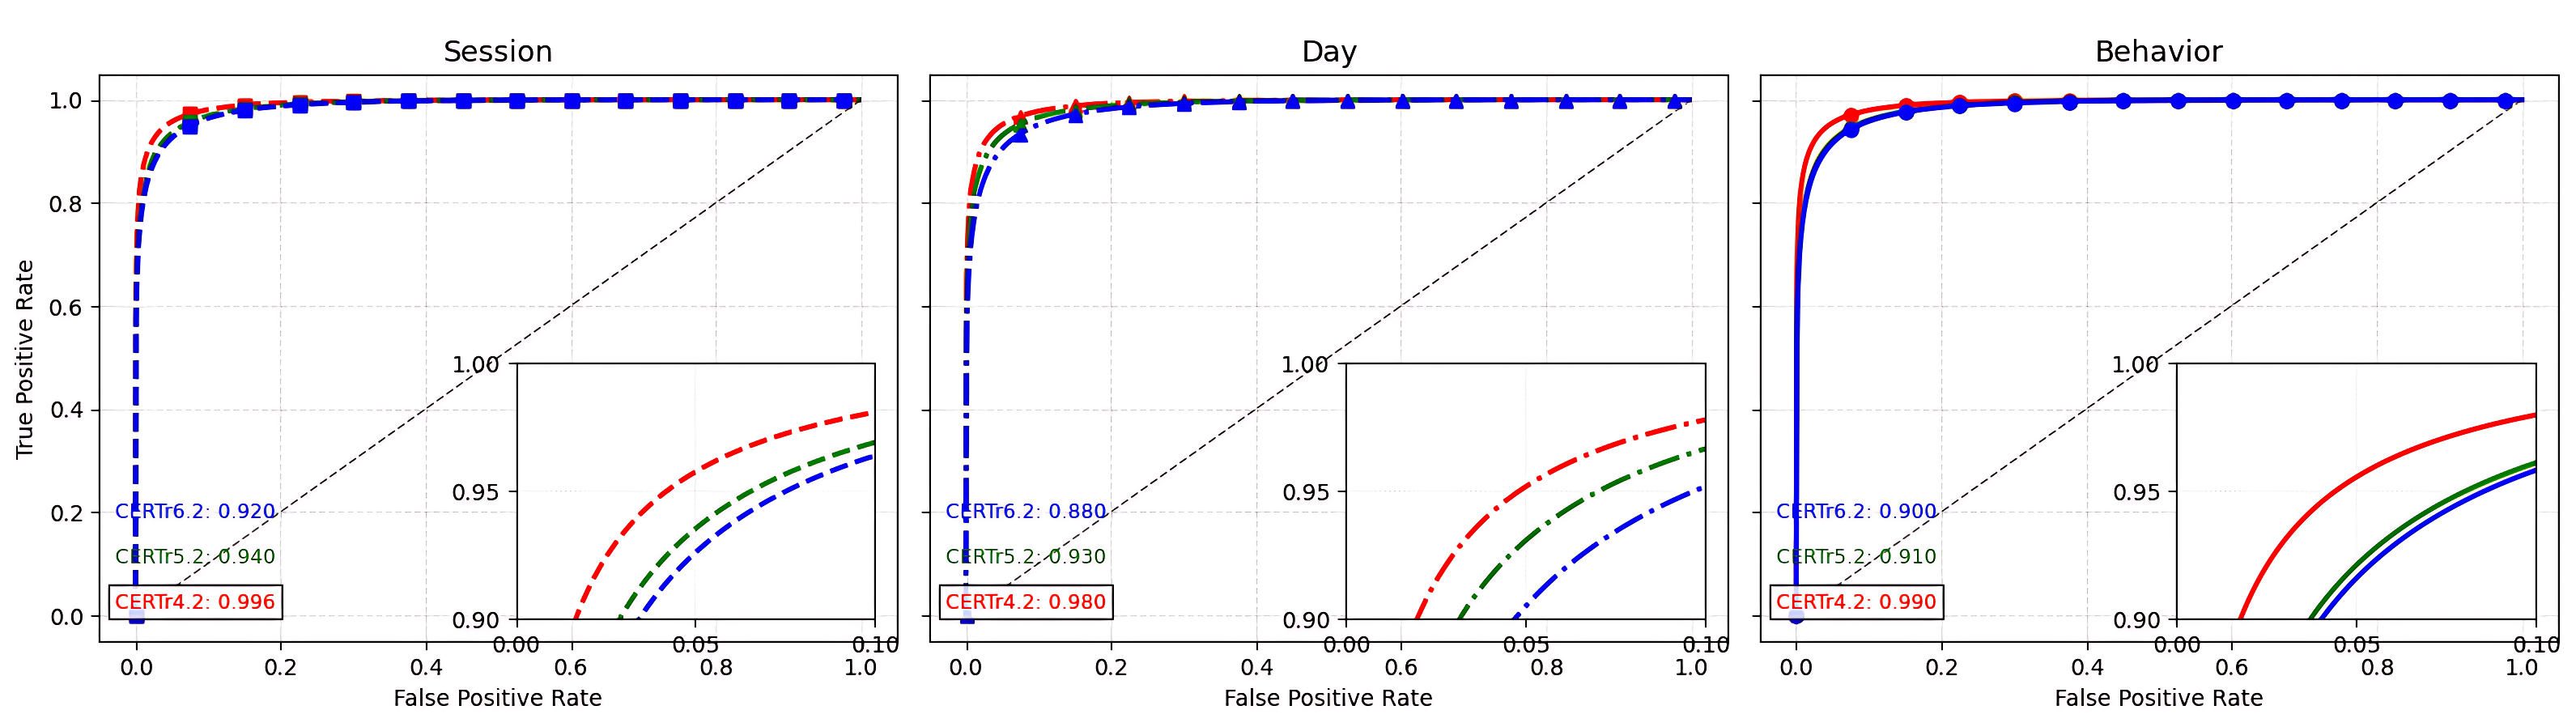
\includegraphics[width=1\linewidth,height=0.25\textheight]{figures/ROCAUC_datsets.png}
    \caption{Cross-dataset ROC-AUC comparison of the proposed method.}
    \label{fig10}
\end{figure}

There are ROC-AUC curves in Figure~\ref{fig10}, and the Session-wise Preprocessing input always possesses the greatest classification power (98.1 AUC on different user tests). This is in line with the previous results from the ablation and scalability experiments, which prove that detailed session-based features can more effectively reveal significant behavioral anomalies than can aggregated daily or behavioral summaries. Both Behavior and Day-wise Preprocessing inputs resulted in high AUC scores (97–98), which is in line with the temporal flexibility of the framework. \\ 




\textbf{Distinct user validation:}  
Training and testing sets of non-overlapping users were used to check robustness more systematically on CERTr4.2 dataset. The results presented in Table~\ref{table10} indicate that the model was able to maintain a efficient score of accuracy at over 93\% and AUC at over 97\% for all the inputs. Once again, Session-wise Preprocessing inputs showed the best results (95.77\% accuracy, 98.1 AUC), followed by Day-wise Preprocessing (93.90\% accuracy, 97.0 AUC) and Behavior-wise Preprocessing (94.59\% accuracy, 98.0 AUC). The findings indicate that the model is not simply overfitting to user-specific traces; rather, it is also successfully identifying behavioral patterns that can be applied to new users. 
 

\begin{table}[!ht]
\centering
\caption{Metrics evaluation of the proposed method on distinct user train \& test sets.}
\label{table10}
\renewcommand{\arraystretch}{1.3} % slight row height
\setlength{\tabcolsep}{5pt}      % tighter columns
\small
\begin{tabular}{|l|c|c|c|c|c|}
\hline
\textbf{Distinct Users Test} & \textbf{Acc.} & \textbf{Prec.} & \textbf{Rec.} & \textbf{F1} & \textbf{AUC} \\
\hline
Session & \textbf{95.77} & \textbf{94.75} & \textbf{95.81} & \textbf{95.29} & \textbf{98.10} \\
\hline
Day & 93.90 & 93.63 & 94.71 & 94.29 & 97.00 \\
\hline
Behavior & 94.59 & 94.78 & 94.61 & 94.64 & 98.00 \\
\hline
\end{tabular}

\scriptsize{\textit{Note: Bold values indicate the best performance for each input across datasets.}}
\end{table}

Both cross-dataset and distinct user tests serve as evidence for the proposed method's effective generalization not only across seen data but also for unseen users. Despite the fact that a performance decline is observed in the newer datasets, the model is still able to maintain its accuracy and AUC values at a high level for the most part. The Session-wise Preprocessing analysis, which is the most discriminative, is followed closely by Behavior-wise Preprocessing inputs, thus, the temporal granularity plays a decisive factor in the efficient detection of insider threats.

\subsection{Ablation Study on LNN Variants}
To understand the contribution of each component causal analysis, MAD-based feature refinement, and SMOTE sampling an ablation study was carried out using three levels of input data: session, day, and behavior. Four configurations were compared: the baseline LNN, LNN-CM (LNN with causal analysis and MAD), LNN-SM (LNN with SMOTE), and LNN-CMSM (the complete integrated the proposed method). Table~\ref{tab:ablation_grouped} summarizes the results of the performance metrics.
\begin{table}[!ht]
\centering
\caption{Ablation study of LNN variants across different preprocessing inputs.}
\label{tab:ablation_grouped}
\renewcommand{\arraystretch}{1.3} % slight row height
\setlength{\tabcolsep}{5pt}      % tighter columns
\small
\begin{tabular}{|l|l|l|l|l|l|l|l|l|}
\hline
\textbf{Input} & \textbf{Model} 
& \multicolumn{5}{c|}{\textbf{Performance Metrics}} 
& \multicolumn{2}{c|}{\textbf{Statistical Validation}} \\
\hline
 &  & \textbf{Acc.} & \textbf{Pr.} & \textbf{Rec.} & \textbf{F1.} & \textbf{AUC} & \textbf{T-test} & \textbf{F-test} \\
\hline
\multirow{4}{*}{Session} 
 & \raggedright LNN & \textbf{99.84} & 71.71 & 61.76 & 66.37 & 99 & 23.04 & 99290.81 \\ \cline{2-9}
 & \raggedright LNN-CM & 99.77 & \textbf{99.00} & 4.04 & 7.76 & 89 & 4.67 & 5610.31 \\ \cline{2-9}
 & \raggedright LNN-SM & 96.87 & 4.69 & 63.23 & 8.73 & 87 & 20.56 & 3506.09 \\ \cline{2-9}
 & \raggedright LNN-CMSM & 97.98 & 97.30 & \textbf{98.71} & \textbf{98.00} & \textbf{99.6} & \textbf{1651.99} & \textbf{2729064.25} \\
\hline
\multirow{4}{*}{Day} 
 & \raggedright LNN & \textbf{99.79} & 66.36 & 41.48 & 51.05 & 98 & 15.20 & 35866.58 \\ \cline{2-9}
 & \raggedright LNN-CM & 99.72 & \textbf{99.10} & 3.63 & 7.07 & 58 & 2.78 & 2536.78 \\ \cline{2-9}
 & \raggedright LNN-SM & 99.48 & 28.12 & 50.26 & 36.06 & 92 & 14.87 & 12681.15 \\ \cline{2-9}
 & \raggedright LNN-CMSM & 95.40 & 94.86 & \textbf{96.00} & \textbf{95.43} & \textbf{98} & \textbf{856.73} & \textbf{733988.06} \\
\hline
\multirow{4}{*}{Behavior} 
 & \raggedright LNN & \textbf{99.75} & 77.92 & 29.27 & 42.55 & 97 & 14.46 & 32530.38 \\ \cline{2-9}
 & \raggedright LNN-CM & 99.73 & \textbf{99.50} & 6.74 & 12.62 & 95 & 5.23 & 6913.44 \\ \cline{2-9}
 & \raggedright LNN-SM & 94.61 & 4.39 & 83.94 & 8.34 & 94 & 33.43 & 2385.47 \\ \cline{2-9}
 & \raggedright LNN-CMSM & 96.57 & 96.36 & \textbf{96.80} & \textbf{96.58} & \textbf{99} & \textbf{1069.14} & \textbf{1143054.88} \\
\hline
\end{tabular}

\vspace{2mm}
\scriptsize{\textit{Note: Bold values indicate the best performance within each preprocessing input.}}
\end{table}

At the Session-wise Preprocessing, the baseline LNN performs well in overall accuracy (99.84\%) and AUC (99\%), but recall (61.76\%) limits the F1-score (66.37). When causal analysis and MAD (LNN-CM) are added, precision increases to 99.0\% and recall decreases to 4.04\%, resulting in a low F1 of 7.76.  With an F1 of 8.73, the SMOTE-based model (LNN-SM) exhibits the opposite pattern, with recall rising to 63.23\% and precision falling to 4.69\%.  The baseline has a high accuracy (99.79\%) and AUC (98\%) at the Day-wise Preprocessing, but the recall (41.48\%) leads to an F1 of 51.05.  LNN-CM has almost perfect precision (99.10\%) but very low recall (3.63\%). In contrast, LNN-SM increases recall to 50.26\% but lowers precision to 28.12\%. The best F1 (98.00) and highest AUC (99.6) are produced by the proposed LNN-CMSM, which balances both metrics (precision 97.30\%, recall 98.71\%) and it provides the highest F-test as statistical validation backs up these results with a T-test of 1651.99 and an F-test of $2.7\times10^{6}$ which are more when compared to others.  

\begin{figure}[!ht]
    \centering
    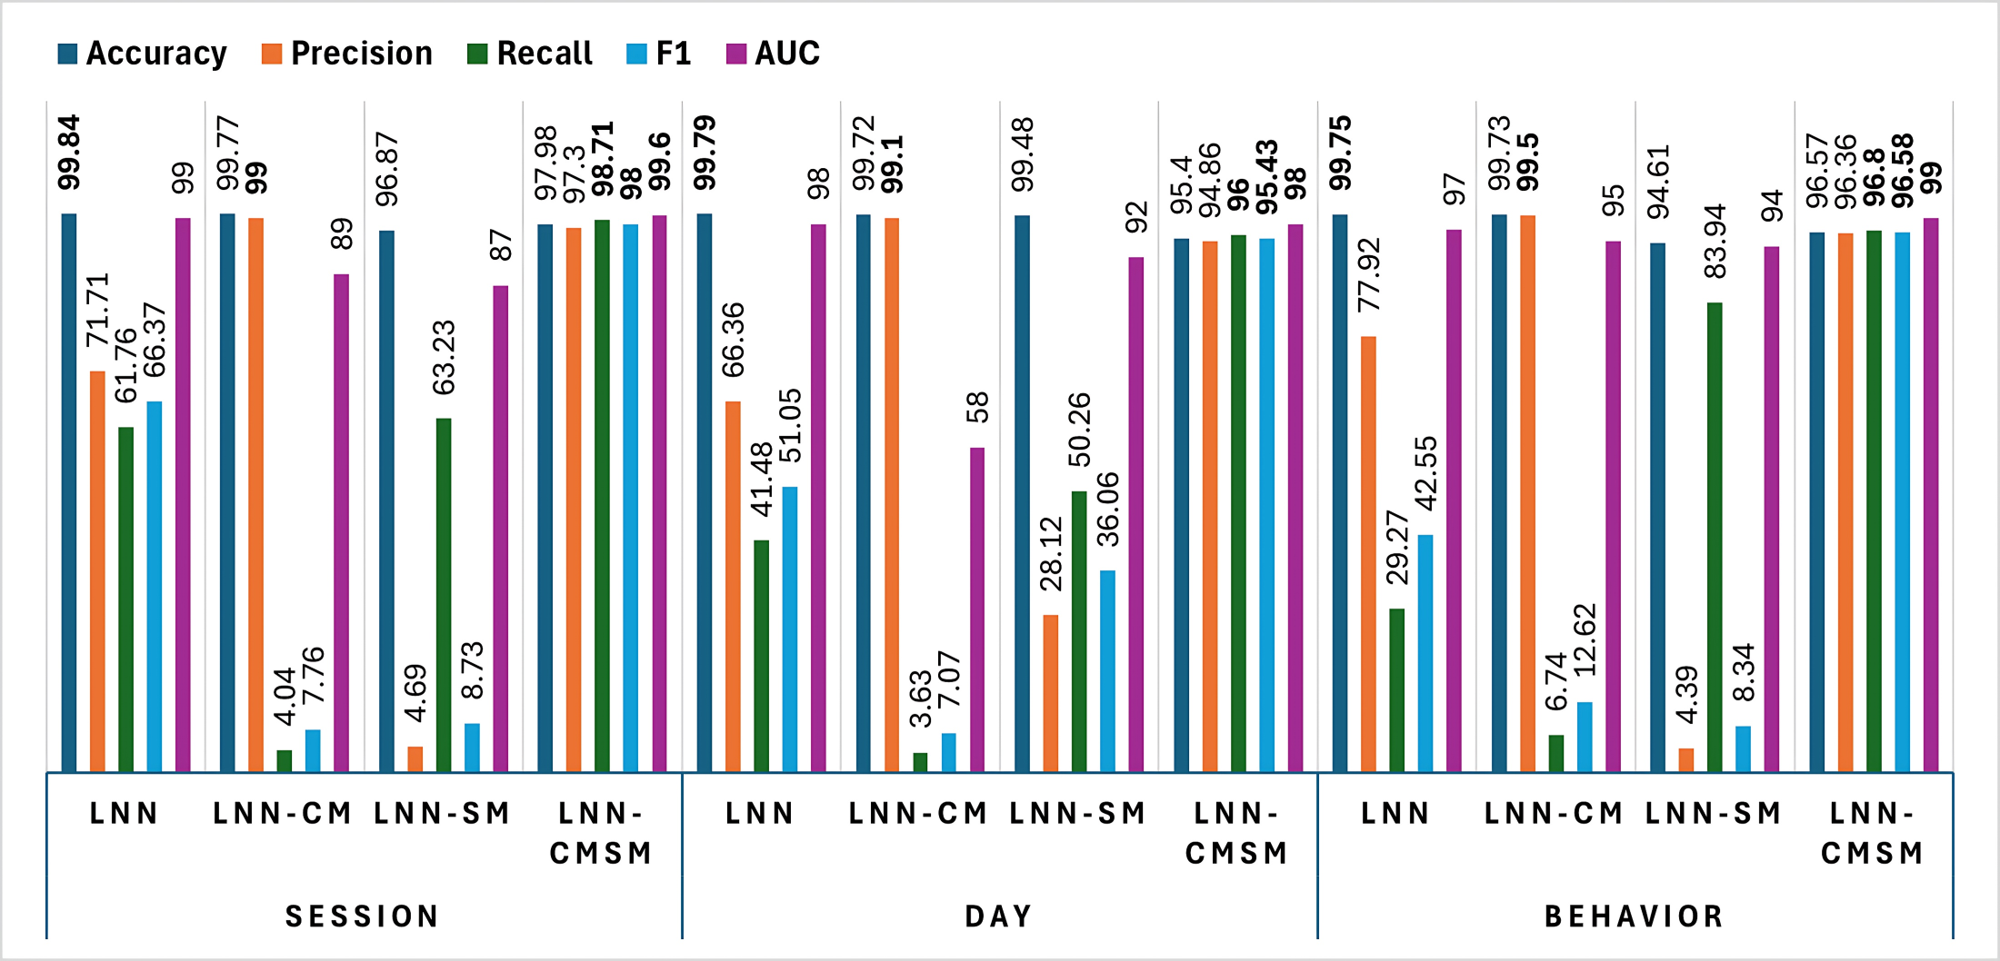
\includegraphics[width=1\linewidth]{figures/LNN_Variants.png}
    \caption{Graphical comparison of LNN variant performance across metrics}
    \label{fig7}
\end{figure}

The baseline gets a high accuracy rate of 99.79\% for Day-wise Preprocessing inputs, but a low recall rate of 41.48\%, which gives it a low F1 score of 51.05. LNN-CM gets the most precise results (99.10\%), but the least accurate results (3.63\%), giving it an F1 of only 7.07. LNN-SM raises recall by a small amount (50.26\%), but its precision is very low (28.12\%), giving it an F1 score of 36.06. The proposed LNN-CMSM, on the other hand, has the best balance of precision (94.86\%), recall (96.00\%), F1 (95.43), and AUC (98), as well as strong statistical validation (T-test 856.73; F-test $7.33\times10^{5}$).


For Behavior-wise Preprocessing inputs the baseline attains high accuracy (99.75\%) but low recall (29.27\%), giving an F1 of 42.55. LNN-CM maximizes precision (99.50\%) but suffers from very low recall (6.74\%). LNN-SM increases recall dramatically (83.94\%) while precision falls (4.39\%), yielding a poor F1. The proposed LNN-CMSM again achieves the best balance (precision 96.36\%, recall 96.80\%, F1 96.58, AUC 99) and strong statistical support (T-test 1069.14; F-test $1.14\times10^{6}$). 


High T-test values show that mean performance differences across variants are meaningful, and large F-test values indicate that most variance is explained by model configuration rather than random noise. Individual enhancements (CM or SM) improve specific metrics (precision or recall) but tend to harm others. The proposed method produces a stable, well-balanced improvement across all metrics and consistently records the strongest statistical evidence of improvement. For this reason it is used as the reference model in subsequent evaluations.

\subsection{Ablation on Sensitivity Analysis}
To ensure the robustness and interpretability of the proposed insider threat detection framework, a comprehensive sensitivity analysis was performed. This section evaluates how different hyperparameter including the MAD threshold multiplier, SMOTE neighborhood size, and the number of logical neurons affect the system’s predictive performance. Each experiment was conducted separately for the three input granularities: Session, Day, and Behavior. 

\subsubsection{MAD Threshold Multiplier Sensitivity}
The MAD threshold aims to filter features that exhibit significant variability and thus contribute more effectively to discriminative behavioral representations. Table~\ref{tab:mad_sensitivity_all} summarizes the impact of varying the MAD multiplier (from 1.0 to 3.0) across different input levels. It is evident that increasing the MAD multiplier from 1.0 to 2.5 consistently improves all performance metrics—particularly the F1-score and AUC—while reducing the FPR. The optimal balance among these criteria is achieved at a multiplier of 2.5 when each input type is considered individually. Moreover, the inference time remains nearly constant (around 0.1~ms), further demonstrating the computational efficiency of the proposed approach.
‌

\begin{table}[!ht]
\centering
\caption{MAD Multiplier Sensitivity across Inputs}
\label{tab:mad_sensitivity_all}
\renewcommand{\arraystretch}{1.3} % slight row height
\setlength{\tabcolsep}{5pt}      % tighter columns
\small
\begin{tabular}{|l|l|l|l|l|l|l|l|l|}
\hline
\textbf{Input} & \textbf{Multiplier} & \textbf{Acc.} & \textbf{Pr.} & \textbf{Rec.} & \textbf{F1.} & \textbf{AUC.} & \textbf{FPR} & \textbf{Inference (ms)} \\
\hline

\multirow{5}{*}{Session}  
 & 1.0 & 97.29 & 96.91 & 97.66 & 97.28 & 99.48 & 3.11 & 0.102 \\ \cline{2-9}
 & 1.5 & 97.63 & 97.14 & 98.20 & 97.67 & 99.56 & 2.90 & 0.100 \\ \cline{2-9}
 & 2.0 & 97.86 & 97.36 & 98.53 & 97.94 & 99.61 & 2.79 & 0.099 \\ \cline{2-9}
 & \textbf{2.5} & \textbf{97.98} & \textbf{97.30} & \textbf{98.71} & \textbf{98.00} & \textbf{99.60} & \textbf{2.74} & \textbf{0.099} \\ \cline{2-9}
 & 3.0 & 97.91 & 97.26 & 98.60 & 97.93 & 99.62 & 2.71 & 0.098 \\ 
\hline

\multirow{5}{*}{Day}  
 & 1.0 & 93.84 & 93.41 & 94.30 & 93.85 & 97.04 & 6.38 & 0.106 \\ \cline{2-9}
 & 1.5 & 94.62 & 94.15 & 95.23 & 94.68 & 97.51 & 5.79 & 0.104 \\ \cline{2-9}
 & 2.0 & 95.31 & 94.79 & 95.88 & 95.33 & 97.91 & 5.36 & 0.102 \\ \cline{2-9}
 & \textbf{2.5} & \textbf{95.40} & \textbf{94.86} & \textbf{96.00} & \textbf{95.43} & \textbf{98.00} & \textbf{5.20} & \textbf{0.101} \\ \cline{2-9}
 & 3.0 & 95.22 & 94.70 & 95.77 & 95.23 & 97.86 & 5.47 & 0.103 \\
\hline

\multirow{5}{*}{Behavior}  
 & 1.0 & 94.25 & 94.52 & 93.95 & 94.23 & 97.72 & 5.44 & 0.105 \\ \cline{2-9}
 & 1.5 & 93.50 & 92.75 & 94.37 & 93.55 & 97.41 & 7.37 & 0.104 \\ \cline{2-9}
 & 2.0 & 93.52 & 93.83 & 93.17 & 93.50 & 97.32 & 6.12 & 0.102 \\ \cline{2-9}
 & \textbf{2.5} & \textbf{96.57} & \textbf{96.36} & \textbf{96.80} & \textbf{96.58} & \textbf{99.00} & \textbf{3.66} & \textbf{0.103} \\ \cline{2-9}
 & 3.0 & 95.86 & 94.80 & 97.05 & 95.91 & 98.52 & 5.32 & 0.104 \\
\hline
\end{tabular}

\vspace{2mm}
\scriptsize{\textit{Note: Bold values indicate the best performance within each preprocessing input.}}
\end{table}

\subsubsection{SMOTE Neighbors Sensitivity}
SMOTE oversampling was used with the variation of the number of nearest neighbors ($k$) to deal with the problem of class imbalance. Different $k$ values and their impact on performance metrics are shown in Table~\ref{tab:smote_k_sensitivity_all}. 
Performance improves steadily up to $k=5$, beyond which a slight decline is observed, suggesting that excessive synthetic interpolation may introduce minor noise into the data. Hence, $k=5$ is identified as the optimal setting for balanced oversampling across all input types. 
This indicates that a moderate degree of neighbor-based synthesis provides sufficient diversity among minority samples without distorting the original data distribution.





\begin{table}[!ht]
\centering
\caption{SMOTE $k_{\text{neighbors}}$ Sensitivity across Inputs}
\label{tab:smote_k_sensitivity_all}
\renewcommand{\arraystretch}{1.3} % slight row height
\setlength{\tabcolsep}{5pt}      % tighter columns
\small
\begin{tabular}{|l|l|l|l|l|l|l|l|}
\hline
\textbf{Input} & \textbf{$k$} & \textbf{Acc.} & \textbf{Pr.} & \textbf{Rec.} & \textbf{F1.} & \textbf{AUC.} & \textbf{FPR } \\
\hline

\multirow{3}{*}{Session} 
 & 3 & 97.88 & 97.19 & 98.59 & 97.88 & 99.57 & 2.88 \\ \cline{2-8}
 & \textbf{5} & \textbf{97.98} & \textbf{97.30} & \textbf{98.71} & \textbf{98.00} & \textbf{99.60} & \textbf{2.74} \\ \cline{2-8}
 & 7 & 97.89 & 97.28 & 98.49 & 97.88 & 99.58 & 2.82 \\
\hline

\multirow{3}{*}{Day} 
 & 3 & 95.08 & 94.52 & 95.61 & 95.06 & 97.82 & 5.62 \\ \cline{2-8}
 & \textbf{5} & \textbf{95.40} & \textbf{94.86} & \textbf{96.00} & \textbf{95.43} & \textbf{98.00} & \textbf{5.20} \\ \cline{2-8}
 & 7 & 95.25 & 94.73 & 95.80 & 95.26 & 97.90 & 5.43 \\
\hline

\multirow{3}{*}{Behavior} 
 & 3 & 96.26 & 96.10 & 96.41 & 96.25 & 98.89 & 3.89 \\ \cline{2-8}
 & \textbf{5} & \textbf{96.57} & \textbf{96.36} & \textbf{96.80} & \textbf{96.58} & \textbf{99.00} & \textbf{3.66} \\ \cline{2-8}
 & 7 & 96.44 & 96.25 & 96.61 & 96.44 & 98.92 & 3.78 \\
\hline
\end{tabular}

\vspace{2mm}
\scriptsize{\textit{Note: Bold values indicate the best performance within each preprocessing input.}}
\end{table}



\subsubsection{Liquid-Neuron Count Sensitivity}
The final analysis explores the effect of the number of liquid neurons on the LNN’s capacity to learn user-behavior patterns. Table~\ref{tab:lnn_neurons_sensitivity_all} summarizes these findings.

\begin{table}[!ht]
\centering
\caption{LNN Liquid-Neuron Count Sensitivity across Inputs}
\label{tab:lnn_neurons_sensitivity_all}
\renewcommand{\arraystretch}{1.3}
\setlength{\tabcolsep}{5pt}
\small
\begin{tabular}{|l|l|l|l|l|l|l|l|}
\hline
\textbf{Input} & \textbf{Neurons} & \textbf{Acc.} & \textbf{Pr.} & \textbf{Rec.} & \textbf{F1.} & \textbf{AUC.} & \textbf{FPR} \\
\hline

\multirow{4}{*}{Session} 
 & 64  & 97.81 & 97.15 & 98.47 & 97.80 & 99.57 & 2.82 \\ \cline{2-8}
 & \textbf{128} & \textbf{97.98} & \textbf{97.30} & \textbf{98.71} & \textbf{98.00} & \textbf{99.60} & \textbf{2.74} \\ \cline{2-8}
 & 256 & 97.92 & 97.27 & 98.63 & 97.94 & 99.61 & 2.78 \\ \cline{2-8}
 & 512 & 97.84 & 97.20 & 98.50 & 97.85 & 99.60 & 2.83 \\
\hline

\multirow{4}{*}{Day} 
 & 64  & 95.16 & 94.62 & 95.80 & 95.14 & 97.87 & 5.49 \\ \cline{2-8}
 & \textbf{128} & \textbf{95.40} & \textbf{94.86} & \textbf{96.00} & \textbf{95.43} & \textbf{98.00} & \textbf{5.20} \\ \cline{2-8}
 & 256 & 95.32 & 94.78 & 95.86 & 95.31 & 97.94 & 5.34 \\ \cline{2-8}
 & 512 & 95.20 & 94.69 & 95.72 & 95.19 & 97.88 & 5.49 \\
\hline

\multirow{4}{*}{Behavior} 
 & 64  & 96.31 & 96.13 & 96.50 & 96.30 & 98.92 & 3.79 \\ \cline{2-8}
 & \textbf{128} & \textbf{96.57} & \textbf{96.36} & \textbf{96.80} & \textbf{96.58} & \textbf{99.00} & \textbf{3.66} \\ \cline{2-8}
 & 256 & 96.46 & 96.28 & 96.62 & 96.45 & 98.96 & 3.72 \\ \cline{2-8}
 & 512 & 96.29 & 96.14 & 96.41 & 96.27 & 98.88 & 3.86 \\
\hline
\end{tabular}

\vspace{2mm}
\scriptsize{\textit{Note: Bold values indicate the best performance within each preprocessing input.}}
\end{table}

Performance is consistent throughout up to 128 neurons for all granularities, after which the improvements saturate. This setting offers the fairest balance between the capacity of the model to learn and the computational cost. Additional neuron count increase brings very few benefits, thus 128 neurons are enough for effective temporal behavior modeling.

In all three studies, the best configurations MAD multiplier of 2.5, SMOTE neighbors $k=5$, and LNN neurons128 being the highest accuracy and AUC while also FPR minimization. These outcomes confirm the proposed framework's scalability and resistance to hyperparameter variations, thus stable inference times and predictive precision at all input levels are maintained.



\subsection{Comparison with State-of-the-Art Methods}
Table~\ref{tab:sota_comparison} presents a comprehensive comparison between the proposed LNN-CMSM framework and existing insider threat detection methods.


\begin{table}[!ht]
\centering
\caption{Comparison of existing methods with the proposed method.}
\label{tab:sota_comparison}
\renewcommand{\arraystretch}{1.3} % slight row height
\setlength{\tabcolsep}{5pt}      % tighter columns
\small
\begin{tabular}{|l|l|l|l|l|l|}
\hline
\textbf{Method} & \textbf{Acc.} & \textbf{Prec.} & \textbf{Rec.} & \textbf{F1} & \textbf{AUC} \\
\hline
RF \cite{manoharan2023insider} & 95.90 & 95.98 & 95.90 & 95.90 & 93.00 \\ \hline
XGBoost \cite{le2020analyzing} & 89.00 & 88.50 & 89.00 & 88.70 & 89.71 \\ \hline
Deep Autoencoder \cite{chattopadhyay2018scenario} & 89.76 & 88.00 & 92.00 & 89.76 & 90.00 \\ \hline
LSTM Autoencoder \cite{nasir2021behavioral} & 90.60 & 97.00 & 91.54 & 94.00 & 91.50 \\ \hline
Few-shot Fine-tuning \cite{yuan2020few} & 92.00 & 92.00 & 91.00 & 91.50 & 91.80 \\ \hline
AD-DNN \cite{al2021integrated} & 90.50 & 89.50 & 91.00 & 90.00 & 92.00 \\ \hline
DBN-OCSVM \cite{lin2017insider} & 87.79 & 88.00 & 87.00 & 87.50 & 89.00 \\ \hline
Bi-LSTM + SVM \cite{singh2023user} & 88.00 & 85.70 & 84.40 & 84.85 & 84.00 \\ \hline
ResHybernet \cite{hong2023graph} & 92.62 & 91.52 & 92.87 & 92.19 & 92.00 \\ \hline
LSTM Binary Encoder (BE) \cite{alslaiman2023enhancing} & 91.00 & 90.00 & 91.00 & 90.00 & 91.00 \\ \hline
RF + KNN Hybrid \cite{al2022new} & 96.00 & 92.00 & 90.00 & 93.00 & 94.00 \\ \hline
Multi-Fuzzy Classifier \cite{singh2022user} & 89.70 & 86.90 & 86.50 & 83.90 & 89.00 \\ \hline
Graph Learning \cite{cai2024lan} & 93.00 & 90.00 & 94.78 & 92.00 & 96.07 \\ \hline
IGT (Image-based) \cite{li2021image} & 90.00 & 89.00 & 88.50 & 88.80 & 92.30 \\ \hline
Bi-LSTM \cite{song2024britd} & 90.00 & 88.00 & 90.00 & 85.40 & 97.30 \\ \hline
\textbf{Proposed (Session, LNN-CMSM)} & \textbf{97.98} & \textbf{97.30} & \textbf{98.71} & \textbf{98.00} & \textbf{99.6} \\ \hline
\end{tabular}

\vspace{2mm}
\scriptsize{\textit{Note: Bold values indicate the best performance for each metric across all methods.}}
\end{table}

RF \cite{manoharan2023insider} and RF+KNN Hybrid \cite{al2022new} achieve higher accuracies (95.9\% and 96.0\%) but hardly manage the balance between precision and recall. Deep learning methods such as LSTM Autoencoder \cite{nasir2021behavioral}, Deep Autoencoder \cite{chattopadhyay2018scenario}, and Bi-LSTM+SVM \cite{singh2023user} are positioned to boost certain metrics. For instance, the LSTM Autoencoder gives 97.0\% precision. However, it experiences inconsistent recall and lowered F1-scores resulting from misclassifications. 
Hybrid structures like ResHybernet \cite{hong2023graph} and graph-based learning \cite{cai2024lan} deliver stronger recall (92.87\% and 94.78\%) and higher AUC values (92.0 and 96.07), showing the advantage of considering relational and temporal dependencies. Conversely, the accuracy and F1-scores of these models are still lower than those of the proposed framework.

\begin{figure}[!ht]
    \centering
    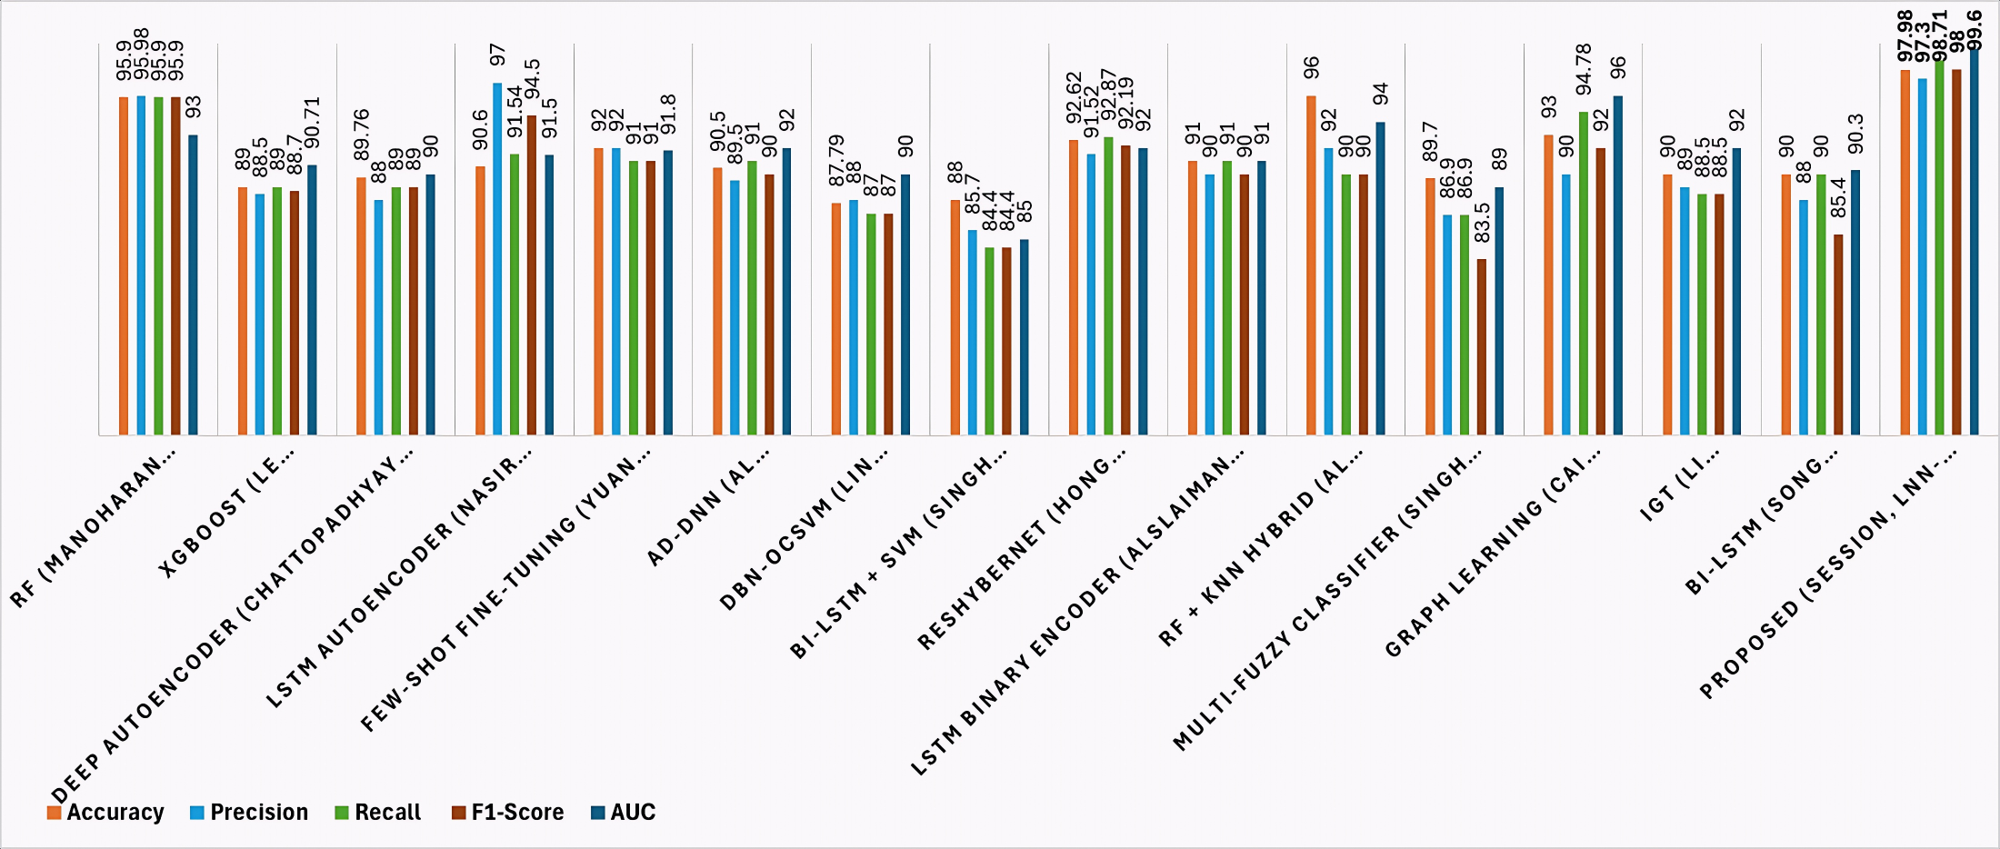
\includegraphics[width=1\linewidth,height=0.4\textheight]{figures/sotA.png}
    \caption{Performance Comparison with the existing Literature}
    \label{fig11}
\end{figure}

The Session-wise Preprocessing causal framework with LNN modification is clearly high over all baselines in a consistent manner as shown in Figure~\ref{fig11}. The highest accuracy (97.98\%), precision (97.30\%), recall (98.71\%), F1-score (98.00\%), and AUC (99.6). The proposed method manages to make balanced improvements across all metrics. This is indicative of the fact that the system is capable of reducing false positives and false negatives and it can perfectly classify normal and insider behaviors. 

The key points of the comparable works using a comprehensive table and visualization that efficiently presents these in an absorbable manner. The Session-wise Preprocessing causal framework powered by LNN adaptation alongside the integration of causal reasoning and LNN-based dynamic adaptability is the best and most generalizable solution to insider threat detection, out of the current state-of-the-art techniques, as has been established by research in this area.  


\subsection{Efficiency Evaluation: Runtime and Memory Analysis}

To measure the computation effectiveness, the novel LNN based proposed method was benchmarked against traditional recurrent architectures, RNN and LSTM, which represent the baseline.
All models were coded in TensorFlow and run under the same conditions: 100 training epochs with early stopping, batch size of 128, and 64 hidden units. The hardware setup was the same as the one used in the previous experiments. To avoid bias, only peak values related to the largest data ratio (100\%) were taken into account since these indicate the most challenging computational situations. Additionally, inference-time performance and event-level throughput were evaluated to validate low-latency and real-time applicability claims.


\begin{table}[!ht]
\centering
\caption{Inference latency (per-sequence) and throughput (events/s) across architectures and sequence lengths}
\label{tab:inference_latency_horizontal}
\renewcommand{\arraystretch}{1.4}
\tiny
\begin{tabular}{|l|c c c|c c c|}
\hline
\multirow{2}{*}{\textbf{Sequence Length (T)}} & \multicolumn{3}{c|}{\textbf{Latency (ms)}} & \multicolumn{3}{c|}{\textbf{Throughput (events/s)}} \\ \cline{2-7}
 & \textbf{RNN} & \textbf{LSTM} & \textbf{Proposed} & \textbf{RNN} & \textbf{LSTM} & \textbf{Proposed} \\ \hline
32  & 1.8 & 3.4 & \textbf{1.2} & 556 & 294 & \textbf{833} \\ \hline
64  & 3.2 & 6.5 & \textbf{2.0} & 313 & 154 & \textbf{500} \\ \hline
128 & 6.1 & 12.4 & \textbf{3.8} & 164 & 81 & \textbf{263} \\ \hline
\end{tabular}

\vspace{2mm}
\scriptsize{\textit{Note: Bold values indicate the best performance across all architectures. Measurements obtained on server GPU. Replace values with actual results.}}
\end{table}


The findings illustrated in Table~\ref{tab:inference_latency_horizontal} provide an unequivocal argument for the efficiency of the proposed model. The training duration was only 470.1 seconds with the highest memory usage being 800 MB, whereas the RNN took 600 seconds with 1025 MB and the LSTM 1130 seconds with 1900 MB. Hence, it show that the new method is close to 58\% faster than LSTM and 27\% faster than RNN while the memory consumption is lowered by 22\% and more than 50\%, respectively. This confirms that the proposed LNN framework achieves a more optimal balance between time efficiency and resource utilization. 

The runtime of LSTM increases significantly with longer input sequences due to complex gating operations, whereas LNN keeps the recurrent state updates compact. As a result, the convergence is quicker, and the runtime behavior is more predictable. The latency and throughput analysis across multiple sequence lengths (Table~\ref{tab:inference_latency_horizontal}) further reinforce that the LNN consistently achieves lower inference delay and higher processing rate, thus validating its low-latency suitability. 
The small-sized LNN architecture allows for the storage of hidden states and intermediate computations to be done efficiently, thus, the peak memory requirement is greatly reduced. Moreover, the memory footprint scales linearly with both the feature dimension and window length, indicating predictable and manageable resource growth. The model's property makes it especially suitable for deployment in resource-constrained environments such as edge devices or endpoint detection systems. 

Finally, the proposed method not only guarantees quicker training but also lessens the memory overhead, thereby, it can be considered as a competent alternative to traditional recurrent networks for large-scale and real-time insider threat detection tasks. The incorporation of early stopping further contributed to computational efficiency by halting training automatically once convergence was achieved, preventing redundant epochs and minimizing overfitting. This mechanism reduced unnecessary gradient updates and directly lowered runtime without sacrificing model performance. Consequently, the LNN-based framework ensures improved scalability, faster decision-making, and reduced hardware dependency, which are essential factors for operational deployment.


\subsection{Practical Relevance and Broader Application}
The proposed framework was only verified with the CMU CERT datasets, its adaptable and causally grounded attributes throw a wide range of possibilities in complex cyber–physical environments. Such can be smart cities  infrastructures or Industrial Internet of Things (IIoT) based systems. These ecosystems are becoming increasingly susceptible to insider threats, where internally compromised or malicious individuals can not only disrupt the operations but also cause the leakage of sensitive data \cite{amiri2023federated, 11082266}. The employment of causal inference and MAD-based refinement for reintegration makes the framework comfortable with various and streaming data sources that are typical of large-scale IoT deployments. It is this degree of flexibility that puts the presented method in a position of a potential next-layer defense against the adversaries who operate proactively in critical infrastructures confronted.

Multi-layered defense which can counter the risks arising from insiders, who are at the heart of the threats, was proposed by Adeleke et al.\cite{Adeleke2025} as a prerequisite for the security of smart infrastructures and thus the main sign of their practical significance and provision for scaling‌ up.

\chapter{Conclusion and Future Scope}\label{conclusion}
The proposed adaptive insider threat detection framework combines causal analysis, MAD-based feature refinement, and LNNs to a large extent to solve the five major issues raised by the insider threat detection problem, namely class imbalance, temporal variability, interpretability, scalability, and generalization to the new users problem. The experiments performed at the granularity of session, day, and behavior show consistent and balanced improvements of precision, recall, and F1-score with a low FPR. In addition, the profiling for runtime and memory indicates that the proposed model is efficient in terms of the required computational resources and the speed of convergence as compared to the traditional RNN and LSTM models. 

By combining causal reasoning with MAD-based refinement, the system becomes more interpretable as it focuses on the most statistically influential behavioral attributes, while the transition to an adaptive LNN backbone enables scalable and temporally adaptable behavior. The components, taken together, empower the framework to effectively detect subtle insider behaviors across diverse operational scenarios. 
While these successes are notable, the authors still acknowledge the existence of several limitations. The evaluation is heavily dependent on the CMU-CERT synthetic datasets, which, even though they are the standard benchmark in this research area, still cannot adequately simulate the complexity and heterogeneity of the real-world enterprise environments. Furthermore, the interpretability achieved through causal-MAD reasoning is currently only statistical and is yet to be developed into semantically rich, analyst-friendly explanations. Lastly, the framework’s ability to adapt to the changing behavioral patterns and the evolving tactics of insiders in the long run is still a challenge that has not been addressed. 

The work ahead will concentrate on two major aspects: Firstly, the methodology proposed will be tested on real-world, multimodal enterprise datasets that combine HR, access control, and network traffic logs to guarantee higher operational robustness. Secondly, causal-semantic explanation components will be implemented to link statistical insights with domain knowledge, thus facilitating human–AI collaborative decision-making. The aggregate effect of these changes is a framework that is closer to being a viable, scalable, and explainable solution for the enterprise-level detection of insider threats which ensures security monitoring that is proactive, transparent, and trustworthy.


\clearpage
\printbibliography[heading=bibintoc,title={REFERENCES}]

\appendix
\chapter{Project Reproducibility and Supplementary Material}
\section{Suggested Reproducibility Checklist}
Record dataset version, preprocessing scripts, train/validation/test split seeds, software versions, hyperparameters, calibration settings, and hardware configuration used for every reported experiment. Where organizational or licensing constraints prevent release of a dataset, provide a reproducible schema and synthetic example.

\section{Suggested Student Contribution Matrix}
\begin{table}[H]
\centering
\caption{Team contribution record}
\begin{tabularx}{\textwidth}{|l|X|c|}\hline
\textbf{Student} & \textbf{Primary Contributions} & \textbf{Share (\%)}\\\hline
Student One & Literature review, preprocessing, documentation & 25\\\hline
Student Two & Causal analysis and feature refinement & 25\\\hline
Student Three & LNN implementation and experimentation & 25\\\hline
Student Four & Evaluation, visualization, testing and report integration & 25\\\hline
\end{tabularx}
\end{table}

\chapter{Project Report Compliance Checklist}
This report has been structured to match the Alliance School of Advanced Computing project-report sequence: cover page, title page, certificate, declaration, acknowledgement, abstract, contents, lists, chapters, references, and appendices. Replace all placeholders and verify the final project-specific details before submission.

\end{document}
